\documentclass{MScthesisITEM}

% this package is just to generate text for demo-purposes

\usepackage{blindtext}
\usepackage{mathtools} % math packages
\usepackage[siunitx]{circuitikz}
\usepackage{todonotes}
\usepackage{hyperref}
\usepackage{subcaption}
\usepackage{listings}
\usepackage{wrapfig}
\usepackage{pgfplots}
\usepackage{filecontents}
\usepackage{url}

%\pgfplotsset{compat=1.11}

\lstset{
	numbers=left,
	stepnumber=1, 
	numbersep=5pt,
	showspaces=false,
	showstringspaces=false,
	showtabs=false,
	basicstyle=\footnotesize, 
	numberstyle=\footnotesize, 
	tabsize=2, 
	breaklines=true,
	captionpos=b,}

\title{Side-Channel Attacks on Cryptographic Implementations} % The title of your assignement; NB use \newlinetitle to start a newline
\author{Martin Kirkholt Melhus \& Haakon Garseg Mørk} % Your firstname and lastname
\professor{Stig F. Mjølsnes, ITEM} % Affiliation = ITEM for instance
\supervisor{Markku-Juhani O. Saarinen, ITEM}

%% Uncomment the following in case you want subfigures; note that there will be a warning for the caption package
% \let\subcaption\undefined
% \let\subfloat\undefined
% \usepackage[bf]{caption}
% \usepackage{subcaption}

\DeclareGraphicsExtensions{.pdf,.jpg}
\graphicspath{{./figs/}}

\loadglsentries{glossary}
\makeglossaries

\begin{document}
\selectlanguage{english}
\pagenumbering{roman}
\pagestyle{plain}

%% Only for the project; comment out the line below for the master's thesis; the front page will be generated automatically by DAIM
\titleITEM

%% Only for the master's thesis; for the project report the description is taken from It's Learning and added by the department
% \selectlanguage{english} % Change to 'norsk' if you are writing in Norwegian
% \begin{titlingpage}

\noindent
\begin{tabular}{@{}p{4cm}l}
\textbf{Title:} 	& \thetitle \\
\textbf{Student:}	& \theauthor \\
\end{tabular}

\vspace{4ex}
\noindent\textbf{Problem description:}
\vspace{2ex}

\noindent \Blindtext[2][1]
\vspace{6ex}

\noindent
\begin{tabular}{@{}p{4cm}l}
\textbf{Responsible professor:} 	& \theprofessor \\
\textbf{Supervisor:}			& \thesupervisor \\
\end{tabular}

\end{titlingpage}
% \cleardoublepage

%% There must be an abstract in English, even though the main text is in Norwegian
\selectlanguage{english}
\pagestyle{empty}
\begin{abstract}
What is the problem, what are the goals, results obtained, summary of the discussion of the results and conclusion.

Foreword / Acknowledgments: When, by whom, where thanks etc.
\end{abstract}
\cleardoublepage

%% Only for the master's thesis; if the main text is in English and you can write Norwegian, there must be an abstract in Norwegian as well.
% \selectlanguage{norsk}
% \pagestyle{empty}
\renewcommand{\abstractname}{Sammendrag}
\begin{abstract}
\noindent Sikkerheten til nesten all offentlig nøkkel-kryptografi er basert på et vanskelig beregnbarhetsproblem. Mest velkjent er problemene med å faktorisere heltall i sine primtallsfaktorer, og å beregne diskrete logaritmer i endelige sykliske grupper. I de to siste tiårene, har det imidlertid dukket opp en rekke andre offentlig nøkkel-systemer, som baserer sin sikkerhet på helt andre type problemer. Et lovende forslag, er å basere sikkerheten på vanskeligheten av å løse store likningsett av flervariable polynomlikninger. En stor utfordring ved å designe slike offentlig nøkkel-systemer, er å integrere en effektiv ``falluke'' (trapdoor) inn i likningssettet. En ny tilnærming til dette problemet ble nylig foreslått av Gligoroski m.f., hvor de benytter konseptet om kvasigruppe-strengtransformasjoner (quasigroup string transformations). I denne masteroppgaven beskriver vi en metodikk for å identifisere sterke og svake nøkler i det nylig foreslåtte multivariable offentlig nøkkel-signatursystemet MQQ-SIG, som er basert på denne idéen.

Vi har gjennomført et stort antall eksperimenter, basert på Gröbner basis angrep, for å klassifisere de ulike parametrene som bestemmer nøklene i MQQ-SIG. Våre funn viser at det er store forskjeller i viktigheten av disse parametrene. Metodikken består i en klassifisering av de forskjellige parametrene i systemet, i tillegg til en innføring av konkrete kriterier for hvilke nøkler som bør velges. Videre, har vi identifisert et unødvendig krav i den originale spesifikasjonen, som krevde at kvasigruppene måtte oppfylle et bestemt kriterie. Ved å fjerne denne betingelsen, kan nøkkel-genererings-algoritmen potensielt øke ytelsen med en stor faktor. Basert på alt dette, foreslår vi en ny og forbedret nøkkel-genereringsalgoritme for MQQ-SIG, som vil generere sterkere nøkler og være mer effektiv enn den originale nøkkel-genereringsalgoritmen.  
\end{abstract}
% \cleardoublepage

\selectlanguage{english}% Change to 'norsk' if you are writing in Norwegian

\renewcommand{\abstractname}{Preface}
\begin{abstract}
\noindent \blindtext 
\end{abstract}
\cleardoublepage

% similarly you may add a separate acknowledgments page

\tableofcontents*
\cleardoublepage

%% include if relevant
\listoffigures
\cleardoublepage

\lstlistoflistings
\cleardoublepage

%% include if relevant
\listoftables
\cleardoublepage

%% include if relevant
% \listofalgorithms
% \addcontentsline{toc}{chapter}{List of Algorithms}
% \cleardoublepage

%% include if relevant
% \printglossary[title=List of Symbols, style=long]
% \cleardoublepage
% \glsaddall[]

% include if relevant
\printglossary[title=List of Acronyms,type=\acronymtype] % prints just the list of acronyms
\cleardoublepage

\pagenumbering{arabic}
\pagestyle{ruled}
\chapter{Introduction}\label{chp:introduction} 

\section{Motivation}
In 2014, Genkin et al. presented their work on exploiting low-bandwidth acoustic emanations to extract a full 4096-bit RSA key~\cite{DBLP:conf/crypto/GenkinST14}.
This novel approach opens for a whole new attack vector that has unexplored potential, as the emanations are allegedly able to leak information about what is being executed on the CPU.
In this paper we will verify some of the claims presented by Genkin et al., by setting up and performing the experiments that are outlined, and possibly reproduce the results presented.


\section{Problem and Scope}
The main goal of this paper is to verify the existence of the acoustic side-channel, and reproduce some of the results of~\cite{DBLP:conf/crypto/GenkinST14}.
We build a similar setup to what was presented, and use it to record computers running in different states.
Then we analyze the recorded acoustic emanations, and attempt to relate the CPU operations to the acoustic emanations.

We diverge from the original project description in that we do not emphasize on applications with regard to cryptanalysis.
Rather we explore the extremes of CPU operations, to be able to verify the initial results of Genkin et al.
We rely strictly on empiric evaluation of our results during analysis, and use no statistical correlation models.
This is done despite the fact that it introduces some limitations to our exploration of the side channel, as the proposed attack on the vulnerable RSA implementation would require such a model.
However, the approach is deemed viable due to the results presented in~\cite{DBLP:conf/crypto/GenkinST14}, and it requires a simpler setup.
Thus RSA key extraction is beyond the scope of this paper.

Using this setup we will show that we are indeed successful in reproducing some of the results presented by Genkin et al., by distinguishing between different CPU activities based on the acoustic fingerprint and computer assisted empirical evaluation.

\section{Methodology}
We record the acoustic emanations of known execution patterns.
Then, we represent the acoustic signatures visually in frequency spectrograms, and empirically try to correlate the nature of the spectrograms with the execution patterns.

\section{Outline}
In this paper we will first present related work, and give a short presentation of the background of our work.
Then we will present our experimental setup, first in the form of the instrumentation; then in the form of the code that we execute on the computers during our experiments.
After this has been described in detail we will present our results, and discuss our findings.

\chapter{Background}
\label{chp:background} 

% Present original research and earlier famous side channel attacks 
%    - Early similar attacks on mechanical systems
%    - Paul Coucher papers for perspective
%    - Original research
%    - 
%    - 
Side-channel attacks is not the kind of standard attack like brute-force attack where you try every single combination to crack a cryptographic algorithm, or like a theoretical weakness that you can take advatage of in cryptographic implementations. 
Side-channel attack exploits the physical implementation to gain information about a cryptosystem.
Characteristics a side-channel attack might exploit can be the power consumption, timing information, electromagnetic radiation, information obtained from a storage after deletion or even sound leakage from the target machine.

Covert-channel attack allows the adversary to communicate with two objects in a physical matter that is not supposed to be allowed. An attack like this is useful when the adversary is able to get inside a computer, but not able to communicate with others what he finds. 
If the adversary knows about a channel, he can use this to transfer the knowledge he has learned.
This channel can be a hardware device that is apparently leaking sound in a frequency that humans cannot hear.


\section{Related work}\label{sec:related_work}

\subsection{Acoustic cryptanalysis}\label{sec:acoustic_cryptanalysis}

Acoustic cryptanalysis is done by listening to sound that is emitted by computers. 
Computers leaks sound from Hz to several hundred kHz. 
\todo{Write something more.. general stuff about acoustic cryptanalysis}

But there are other ways to do acoustic cryptanalysis. In 2005, some researchers at Berkeley did a research\cite{keystrokes} on recognizing keystrokes on a keyboard by sound. 
This is possible because each key has its own distinct sound. 
After separating the different keystrokes, they used a statistical frequency method to find out which key belonged to which letter. 
To determine the letters, they only had to listen for 10 minutes, i.e. on a typical user that types about 300 characters each minute. 
One method to take advantage of this attack is to create a mobilephone application that enables the microphone and analyses the keystrokes. 

Its also proven that phones and ATMs with mechanical keyboards can be vulnerable for acoustic attacks\cite{KybdEmanation}.

In 2014, a research team at the Tel Aviv University was able to do a full RSA Key (4096-bit) extraction using acoustic cryptanalysis. 
This research is explained in detail at section \ref{sec:original_research}.

\subsection{Data remanence}\label{sec:data_remanence}

Data remanence is remaining representation if digital bits after attempts of deletion or removal of data. 
The recovery of these bits may be due to the technique used to delete or the physical characteristics of the storage media. 
The problem of data remanence was first observed in magnetic media, when it was proven that data could be restored after several times of overwriting. 
This proof is however just a theortical proof. 
Nobody has ever proven to restore bits after been overwritten. 
\todo{Write something more.. general stuff about data remanence}

Earlier it has been shown that for some UV EPROM, EEPROM and Flash devices, information can still be recovered after 100 erase cycles\cite{data_remanence_flash}.


\subsection{Differential fault analysis}\label{sec:differential_fault_analysis}

Differential fault analysis is cryptanalysis based on interpreting fault outputs from a processor exposed to different kinds of environmental exposure like high voltage or current, strong elektromagnetic fields or as simple as high temprature. 
The processor might give fault outputs an adversary can use to find knowledge about the processor state or similar information.


Guo, et al (2012): Invariance-based concurrent error detection for advanced encryption standard\cite{dfa_guo}
\todo{Is this paper something to write about?}

Giraud (2003): DFA on AES\cite{dfa_aes}
\todo{Is this paper something to write about?}

\subsection{Electromagnetic attacks}\label{sec:electromagnetic_attacks}

An adversary can, if located within range, intercept electromagnetic signal emitted by all electronic devices. 
It is not possible to detect this attack, and therefore hard to prevent. 
One of the known attacks is extracting the electromagnetid signals from a computer monitor to reproduce the screen output.
These signals originates from the electron gun that manipulates each pixel\cite{tempest_sans}. 
The stronger a pixel is, the stronger the signal.
PGP includes a secure viewer that prevents exactly these high frequency signals by making softned edges in the fonts.
However, it is said to be very difficult, thus expensive to extract the signals emitted by a computer monitor. 

\subsection{Power analysis}\label{sec:power_analysis}

Electronic devices leaks information about what they are processing through their power consumption.
This leakage can be used to extract secret information like keys used to encryption using differential power analysis (DPA). 

Simple power analysis (SPA) is simply interpreting the power consumption measurements during cryptographioc operations\cite{dpa_kocher}. 

DPA is a more complex way to interpret the power consumption. \todo{write something fancy about DPA}
Paul Kocher: Differential power analysis \cite{dpa_kocher}

\subsection{Timing attacks}\label{sec:timing_attacks}

Here goes related work to timing attacks

SSL Timing attack~\cite{ssl_timing_attack}
Timing attack Diffie-Hellman~\cite{timing_attack_kocher}

\section{Original research - Acoustic Cryptanalysis}\label{sec:original_research}

The original research that we are referring to in this paper, is the RSA Key Extraction via Low-Bandwidth Acoustic Cyptanalysis~\cite{original_paper}, done by Daniel Genkin, Adi Shamir and Eran Tromer.
Their claim is that many computers leaks acoustic noise from its electronic components due to vibration, i.e. coil whine (noise).
Vital components like the CPU requires power dependent on what it is computing.
Hence the theory is that some CPUs leaks acoustic noise about what it is doing.
They use this information to extract a 4096-bit RSA key.

\subsection{Lab setup}\label{sec:lab_setup}

The noise they are trying to record and interpretate is found in different and high frequencies, thus high sensitivity microphones is required. 
They use 3 different microphones from Brüel\&Kjær showed in figure~\ref{fig:bruel_kjaer_mics}

\begin{figure}[h]
	\centering
    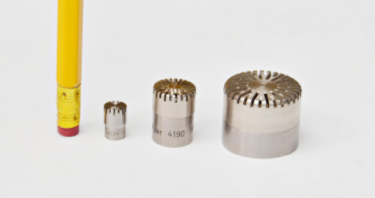
\includegraphics[width=0.4\textwidth]{bruel_kjaer_mics.png}
    \caption{Brüel\&Kjær 4145 (up to 21kHz), 4190 (up to 40kHz) and 4939 (up to 350kHz)~\cite{original_paper}.}
    \label{fig:bruel_kjaer_mics}
\end{figure}



\subsection{Acustic leakage}\label{sec:acustic_leakage}


\subsection{RSA key extraction}\label{sec:rsa_key_extraction}


\chapter{Experimental Setup}
\label{chp:experimental_setup} 

intro..

\section{Microphone selection}\label{sec:microphone_selection}

Our experimental setup uses the Zoom H4n Handy Recorder. 
The recorder is able to record WAV files with a sampling frequency \( {F_{s}} \) of 96kHz and a quantization of 24 bit. We were also able to plug it directly into a computer, thus using it as the standard sound input device. 
However this limited the operating sampling frequency \( {F_{s}} \) to 48kHz.

Since a lot of the information we are looking for is in a frequency range far above the hearing range of the human ear, we require a microphone that can capture these frequencies. 
The frequencies we are able to observe are limited to the Nyqyust frequency.

\begin{equation}\label{eq:nyquist_frequency}
F_{nc} = \frac{F_{s}}{2}
\end{equation}

This means that we are able to study the frequency response up to frequencies of 48kHz using the setup.
In original research, it is claimed that there is information for fingerprinting in this frequency range, thus we should be able to observe the phenomenons.

\subsection{Zoom H4n Configuration}\label{sec:zoom_H4n_configuration}

The Zoom H4n Handy Recorder is set to Sterio Mode.
Further, the sampling frequency is set to 96 kHz and the analog to digital converstion is set to the maximum which is 24 bit.
Further the recorder provides a 237 Hz low cut filter, which is enabled.
These low-frequency frequency responses are not providing information that is critical for looking at the fingerprints and \todo{citation paper; Look at explanation from the original paper} \todo{Low cut filter not working??? Cannot be observed in plots ...} 

Since we do not have a remote controll for the recorder, we have to manually click the record button to start and stop our recordings. 
This means that we are touching the recording device, thus impacting the samples when the contact is happening. 
This is not critical for our setup, as we are recording a time interval of several seconds; only the samples in the timeframe when we are activly starting and stopping the recording are affected by the physical contact. 
However this makes it harder for us to do multiple recordings with the recorder in the exact same place, as touching the device will inevitably cause some slight displacement.

\section{Processing and signal extraction}\label{sec:processing_signal_extraction}

The captured sound is stored in a WAV file.
This file is processed in our self written software, which utilizes libraries such as FFTW \todo{citation here} and libsndfile \todo{citation here}.
The samples are devided into windows \( W \), where \( \lvert W \rvert = 2^{n} \) where \( n \) is a non-zero positive integer.

The WAV file contains a sterio signal, but since our audio source is hardly a sterio source, we only need one of the channels for our furter processing. \todo{Reasoning about why we only need mono} 
In the WAV format, frames representing each sample is stored subsequently, such that the sample \( s_{f,c} \) represents the PCM \todo{Pulse-code modulation abbrevation} response for frame \( f \) channel \( c \). 
Since we have a stereo signal, we have that \( f \in \left [ 1, 2 \right ]  \), and thus the samples are ordered  \( s_{0,0}, s_{0,1}, s_{1,0}, s_{1,1}, ... , s_{n,0}, s_{n,1} \). 
To obtain a mono signal we simply ignore all frames where \( f \neq 0 \).


\section{Capturing audio fingerprint}\label{sec:capturing_audio_fingerprint}

\chapter{Predictable Execution and Mapping to Time Domain}\label{chp4:predictable_execution} 
A prerequisite to analysis of acoustic fingerprints is to have some idea of what is being recorded, to be able to look at the correlation between what is happening, and what was being observed during the same period of time.
In our case this means that we need to know what happening on in the \gls{CPU} for the duration of our recordings.
With this knowledge, we should be able to perform analysis regarding the correlation between what is observed in the acoustic emanations and distinct \gls{CPU} activity.
This chapter will describe how we force predictable \gls{CPU} activity during experiments, and also how we tailor the software run on different architectures to achieve comparable results.
We will also outline our expectations regarding analysis of the acoustic emanations from the experiments.

\section{Selection of Test Cases}
We use several test cases, where the aim is to gradually record increasingly subtle variations in \gls{CPU} activity, and the recordings of these will makes the basis for analysis.
Each of these cases are represented by a utility; a program that is specifically tailored to force the desired \gls{CPU} activity during the experiment.
We will start by oscillating between abnormally high \gls{CPU} loads and a idle system, and eventually we will try to distinguish between the execution of the repeated execution of different distinct microinstructions and specific \gls{CPU} operations.

The following sections will in detail describe the different utilities we use to inflict this \gls{CPU} behavior, and how we wrap the different tokens of predictable executions in a deterministic repeated pattern to be used in later analysis, hence relating the \gls{CPU} behavior to the time domain.

\section{CPU load}\label{chp4:sec:cpu_load}
Our first choice of distinguishable \gls{CPU} activity is in the form of a \gls{CPU} burn utility. 
The idea is that when no programs are running, save the operating system, the activity level of the \gls{CPU} us low. 
However, if the user executes a program that will make all cores on the \gls{CPU} work at close to their full capacity, the internal activity of the \gls{CPU} will change drastically as a consequence of the increased load.
Additionally, the temperature of the \gls{CPU} will increase, hence the name.

All these desired properties are available in the cpuburn collection which can be installed using the debian package manager (using
apt-get install cpuload).\todo{Some citation here (manpage?) potentially http://www.hecticgeek.com/2012/03/cpuburn-cpu-stress-test-ubuntu-linux/}
To be able to relate this to the time domain, we execute the \gls{CPU} burn tool in the pattern described in \autoref{lst:cpuburn_loop_utility}.

\begin{lstlisting}[language=BASH, caption={Mapping execution to the time domain: CPU Burn Utility}, label={lst:cpuburn_loop_utility}]
for i in {1..3}
do
	# burn all cores for 2 seconds
	sleep 1
done
\end{lstlisting}

In a loop, the \gls{CPU} will operate at close to full capacity, then sleep for a second, representing the heavy load state and the idle state.
By recording during execution of this utility, we hope to be able to distinguish between the two states, heavy load and idle, thus be able to observe a repeating pattern with a period of \(3\) seconds, representing the loop.

For the Raspberry Pi, we use the sysbench~\cite{url:sysbench_wiki} package to generate CPU load. 
This package has a benchmarking tool for ARM \gls{CPU}s, which is used to generate \gls{CPU} load.

\section{Microinstructions}\label{chp4:sec:microinstructions}
\todo{Ingress}


\subsection{Mapping to Time Domain}\label{chp4:sec:mapping_to_time_domain}
The next utility is used to force reliable execution of different microinstructions and \gls{CPU} operations.
Genkin et al. suggest that looping through a set of microinstructions that are repeated over an observable period of time, should result in a distinguishable acoustic fingerprint for each \gls{CPU} operation.
We want an utility that lets us do a similar experiment, and possibly achieve similar results.

Since we are using sampling frequencies in the kHz-range and processors operate on frequencies in the GHz-range, it is futile to try to capture the fingerprint of a single clock cycle representing the execution of a specific microinstruction. 
This limitation can be overcome by repeating the same instruction for a longer period of time, such that every \(\Delta t\) seconds, a new instruction will start executing, and this instruction will execute in a loop until it is replaced after another \(\Delta t\) seconds.
With \(n\) different instructions, one pass through all instructions will take \(T = n \times \Delta t\) seconds.
We want to repeat the loop more than once, so that we can look not only for a change from one lastingly stable signal every \(\Delta t\) seconds, but also a repeating pattern every \(T\) seconds, representing the loop over all instructions.

The microinstruction repetition pattern used in this utility is given in \autoref{lst:microinstruction_loop_utility}

\begin{lstlisting}[language=BASH, caption={Mapping execution to the time domain: Microinstruction loop utility.}, label={lst:microinstruction_loop_utility}]
for i in {1..3}
do
	for j in {1..n}
	do
		# run instruction j for 0.33 seconds
	done
done
\end{lstlisting}

The \gls{CPU} operations we will loop are the MUL, ADD and NOP microinstructions as well as memory access with forced L1 and L2 cache miss.
The following subsections will go into further detail on how timely and predictable execution is achieved in all four cases for both ARM and x86 architectures.


\subsection{Memory Access and Predictable Cache Miss}\label{chp4:subsec:MEM_operation}
The memory dereference (MEM) operation's performance with regard to speed depends heavily on if the target is cached or not. 
If cache hit occurs in the L1 or L2 cache, the lookup time is much lower than if the value is read from the \gls{RAM}.
We want to achieve an execution sequence where the \gls{CPU} constantly has to go all the way to the RAM to fetch values.


As it turns out, list access loads and stride access loads are a good generator of cache misses~\cite{DBLP:conf/micro/OzawaKN95}.
Unfortunately, modern processors are putting great effort into predict memory accesses; constant stride load patterns can easily be detected in hardware~\cite{DBLP:journals/taco/LeeKV12}, and the data can be prefetched causing few to zero cache misses.
For this reason, we cannot rely on simple mechanisms such as sequential memory access using a stride bigger than the size of the cache.
Luckily the existence of hardware performance counters made available in the Linux operating system allow us to evaluate our approach to the MEM operation. 
Performance counters are a set of hardware registers that can be used to count events such as cache misses during the execution of a program, without impacting the execution~\cite{url:perf_wiki}.
Therefore, we are able to benchmark our approach, and verify if we successfully bypass prediction and prefetching mechanisms.

We make two programs; \(A\), which randomly resolves \(n = 1000\) indexes in an array that is several orders of magnitude bigger than the L2 cache of the targeted CPU; and \(B\), which is identical to \(A\), save the fact that it deterministically resolves subsequent indexes.
During the course of execution, \(A\) should to suffer approximately \(k+n\) cache misses, while \(B\) should suffer only \(k\), due to successful stride prediction.
Here \(k\) represents the baseline cache misses suffered for running the parts in some section of the program required to set up the loop, and \(n\) represents the amount of cache misses suffered from resolving indexes in the array.
If this condition holds, we can argue that the program \(A\) should cause \(n\) more cache misses than \(B\) and thus reliably executes the MEM operation. 

\todo{Make inverse CDF and fix dotted line. Do flat lower limit removal in data set.}
\begin{figure}
    \begin{subfigure}{0.5\textwidth}
        \centering
        \resizebox{0.9\textwidth}{!}{
            \begin{tikzpicture}
                \begin{axis}[
                    %title={Cache Miss Probability Distribution},
                    xlabel={$\Delta C$},
                    ylabel={$p$},
                    legend pos=north east,
                    legend style={font=\tiny},
                    grid style=dashed,
                    ymajorgrids=true,
                    ymode=log,
                    %ymin=0, ymax=1,
                ]
                \addplot table [smooth,dotted,mark=none,y=p,x=C,col sep=comma] {data/prob-density-dell.dat};
                \addlegendentry{Dell Latitude D430}
                \end{axis}
            \end{tikzpicture}
        }
        \caption{Dell Latitude D430}
    \end{subfigure}
    \begin{subfigure}{0.5\textwidth}
        \centering
        \resizebox{0.9\textwidth}{!}{
            \begin{tikzpicture}
                \begin{axis}[
                    %title={Cache Miss Probability Distribution},
                    xlabel={$\Delta C$},
                    ylabel={$p$},
                    legend pos=north east,
                    legend style={font=\tiny},
                    grid style=dashed,
                    ymajorgrids=true,
                    ymode=log,
                    %ymin=0, ymax=1,
                ]
                \addplot table [dashed,mark=none,y=p,x=C,col sep=comma] {data/prob-density-lenovo.dat};
                \addlegendentry{Lenovo Thinkpad T60p}
                \end{axis}
            \end{tikzpicture}
        }
        \caption{Lenovo Thinkpad T60p}
    \end{subfigure}
    \caption{Empirical probability distribution of suffered cache misses - \(\Delta C\) - when running the MEM benchmark.}
    \label{fig:mem_benchmark}
\end{figure}

We ran \(A\) and \(B\) \(1000\) times, measuring the number of cache misses \(c_A\) and \(c_B\) suffered by \(A\) and \(B\).
Then we look at the difference in cache misses \(\Delta C_i = c_{A_i} - c_{B_i}\) for every run \(i \in [1, 1000]\).
The results are given in \autoref{fig:mem_benchmark}, and represent the results for our two target laptops; a Lenovo T60p laptop with a Intel Centrino Duo \gls{CPU}; and a Dell Latitude D430 laptop also with a Intel Centrino Duo \gls{CPU}.
They clearly show that the probability of observing the expected \(\Delta C\) close to \(1000\) prevalent for both of the computers.
This is good enough to satisfy our condition, as the amount of cache misses suffered also strictly higher in \(A\) as compared to \(B\).
Our MEM utility program is successfully bypassing the \gls{CPU}s best efforts of hardware prefetching and stride prediction.
For code-level details as to how the benchmark was conducted, see~\autoref{apx:mem_benchmark}.




\subsection{MUL, ADD and NOP execution on Different Architectures}\label{chp4:subsec:MUL_ADD_NOP_instructions}
The three native microinstructions that we look at are MUL, ADD, and NOP.
To achieve the repeated execution of these instructions over time, we repeat the assembly code for each instruction \(1000\) times in a loop.
This ensures that the targeted instructions are prevalent, and reduce the impact of the required instructions to perform the eventual loop, and tracking the overall duration.

\newsavebox{\MEMfigure}
	\begin{lrbox}{\MEMfigure}%store first listing
	\begin{lstlisting}[language={[x86masm]Assembler}]
		mov $0, %eax;
		mov $1, $ebx;
		mul %eax;
	\end{lstlisting}
\end{lrbox}

\newsavebox{\ADDfigure}
	\begin{lrbox}{\ADDfigure}%store first listing
	\begin{lstlisting}[language={[x86masm]Assembler}]
		mov $0, %eax;
		mov $1, $ebx;
		add %ebx, %eax;
	\end{lstlisting}
\end{lrbox}

\begin{figure}[h]
    \begin{subfigure}{0.5\textwidth}
        \centering
        \usebox{\MEMfigure}
        \caption{MEM}
    \end{subfigure}
    \begin{subfigure}{0.5\textwidth}
        \centering
        \usebox{\ADDfigure}
        \caption{ADD}
    \end{subfigure}
	\caption{The setup code for the NOP and MEM instructions. The instruction on line no. 3 is repeated \(1000\) times.}
	\label{lst:x86_add_mem}
\end{figure}

The NOP operation is represented by rep; nop; repeated \(1000\) times; for the MEM and ADD instructions, see \autoref{lst:x86_add_mem}.


\subsection{Expectations regarding acoustic fingerprints}
The utility is combining the MEM operation, as described in \autoref{chp4:subsec:MEM_operation} and the MUL, ADD and NOP-loops which are described in \autoref{chp4:subsec:MUL_ADD_NOP_instructions}.
Executing the four operations in the pattern given in \autoref{lst:microinstruction_loop_utility}, the goal is to observe repeating patterns in the acoustic emanations of the \gls{CPU}s during execution of the utility.
More precisely, we will look for periodic patterns that with a duration in time \(t\) of \(0.33\) seconds, representing individual operations. 
If we can see such patterns with a period of \(4t = 1.33\) seconds, the same as that of our outer loop, it would suggest that the emanations are be caused by the \gls{CPU} performing the operations forced by our utility.
Thus we can argue that we are in fact able to distinguish between such low level operations based purely on the acoustic fingerprint. 



\section{Decryption}\label{chp4:sec:decryption}
Genkin et al. suggest that it is possible to distinguish between the different steps involved in a decryption using a 4096-bit RSA key.
For our decryption utility, we will use the same key size, and perform decryption. 
We use the GnuPG 1.4.15~\cite{url:GnuPG_1.4.15} library as it has the suggested vulnerabilities found in GnuPG versions up to 1.4.15\cite[Sec.~9.1]{DBLP:conf/crypto/GenkinST14}. 

The cipher text being decrypted is the result of encrypting a 4.2MB WAV format sound file, using a 4096-bit RSA key with the vulnerable version of GnuPG.
Essentially we are using the same encryption and decryption method, key-size and key generation as Genkin et al. 

To be able to relate the decryption to the time domain, we execute the decryption according to the pattern given in \autoref{lst:decryption_loop_utility}

\begin{lstlisting}[
language=BASH, 
caption={Mapping execution to the time domain: Decryption loop utility.}, 
label={lst:decryption_loop_utility}]
for i in {1..3}
do
    sleep 1
    # perform decryption
done
\end{lstlisting}

The pause between each decryption may resolve in a pattern that can be observed during analysis of the acoustic emanations, by allowing us to relate what is happening to the time domain, in the sense that we know the duration of each sleep.
The duration of a single decryption can also be measured, although it will differ on different computers.
Therefore we are left with a clear idea of what to search for during analysis.

\chapter{Applications in Cryptanalysis}
\label{chp:application_in_cryptanalysis} 

\section{The vulnerability in GnuPG v1.4.15}\label{sec:vulnerability_gnupg}

\subsection{Subsection}\label{sec:first_ssection}


\section{The attack}\label{sec:attack}


\section{Chosen plaintext}\label{sec:chosen_plaintext}

\begin{wrapfigure}{r}{1\textwidth}
    \centering
    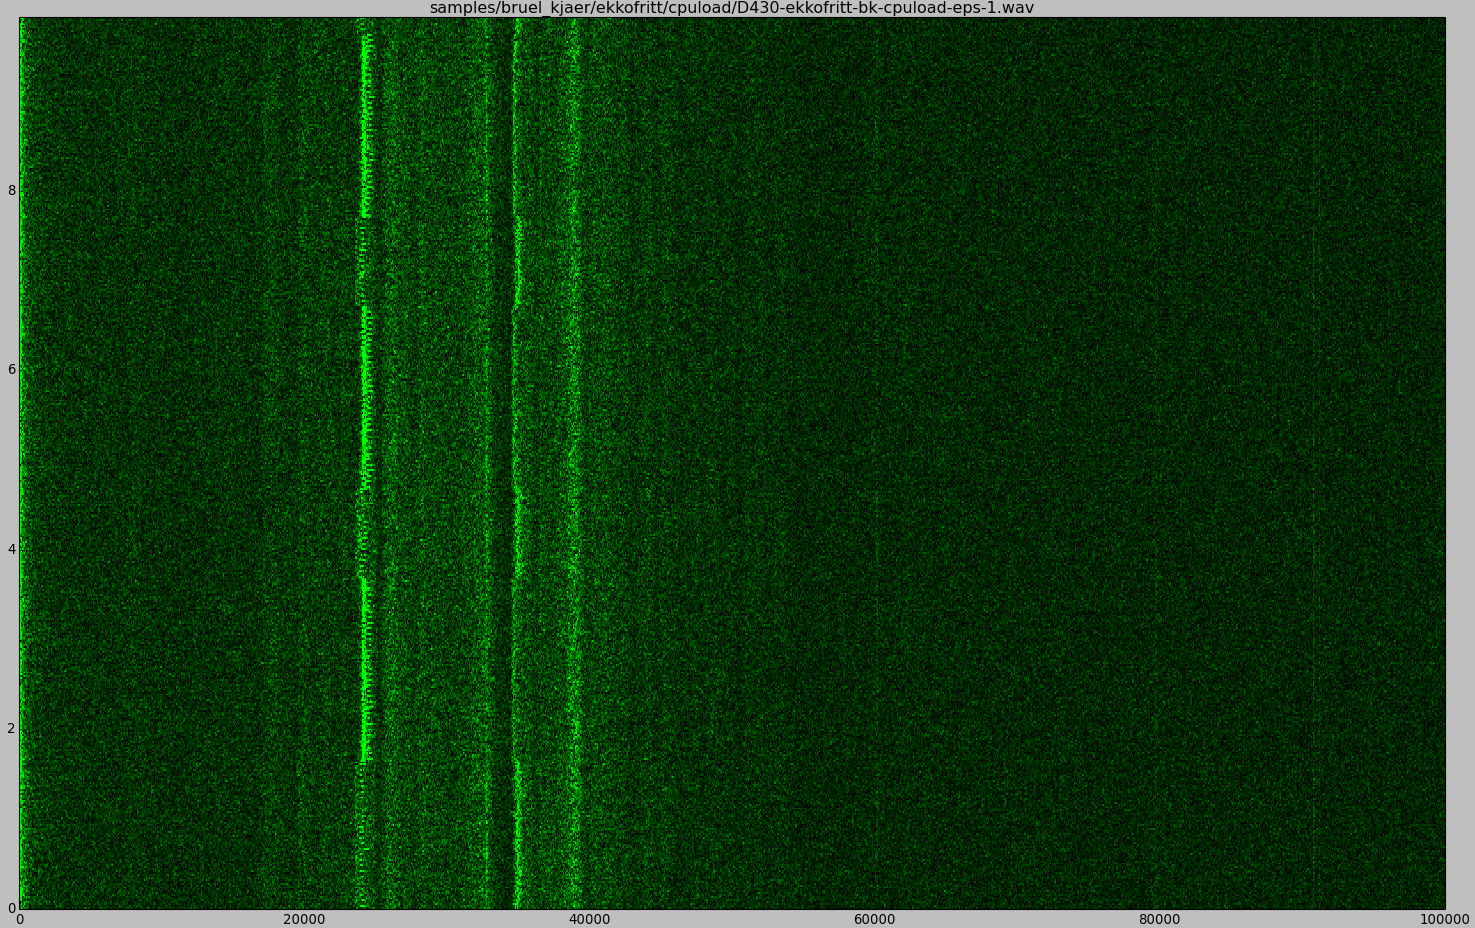
\includegraphics[width=1\linewidth]{D430-ekkofritt-bk-cpuload-eps-1.png}
    \caption{Acoustic recording (10 sec, 0-100kHz) of the Dell D430 when running a full CPU load. The recording was made in an anechoic chamber using the Brüel\&Kjær 4939 microphone with the NI myDAQ. }
    \label{fig:D430-ekkofritt-bk-cpuload-eps-1}
\end{wrapfigure}

\begin{wrapfigure}{r}{1\textwidth}
    \centering
    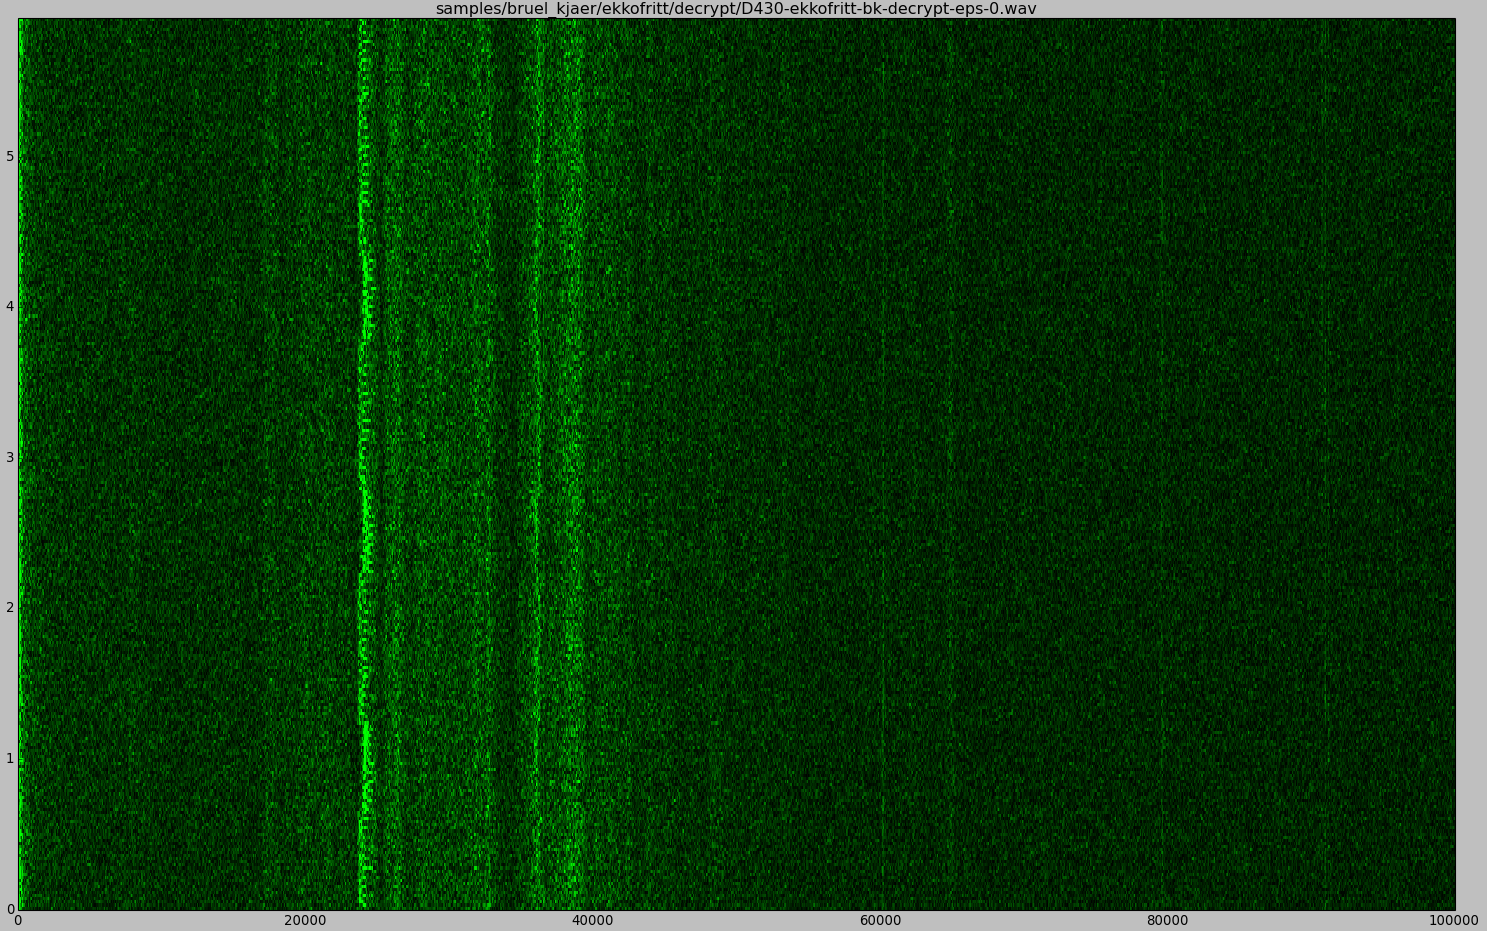
\includegraphics[width=1\linewidth]{D430-ekkofritt-bk-decrypt-eps-0.png}
    \caption{Acoustic recording (6 sec, 0-100kHz) of the Dell D430 when running a dycrypt. The recording was made in an anechoic chamber using the Brüel\&Kjær 4939 microphone with the NI myDAQ. }
    \label{fig:D430-ekkofritt-bk-decrypt-eps-0}
\end{wrapfigure}

\begin{wrapfigure}{r}{1\textwidth}
    \centering
    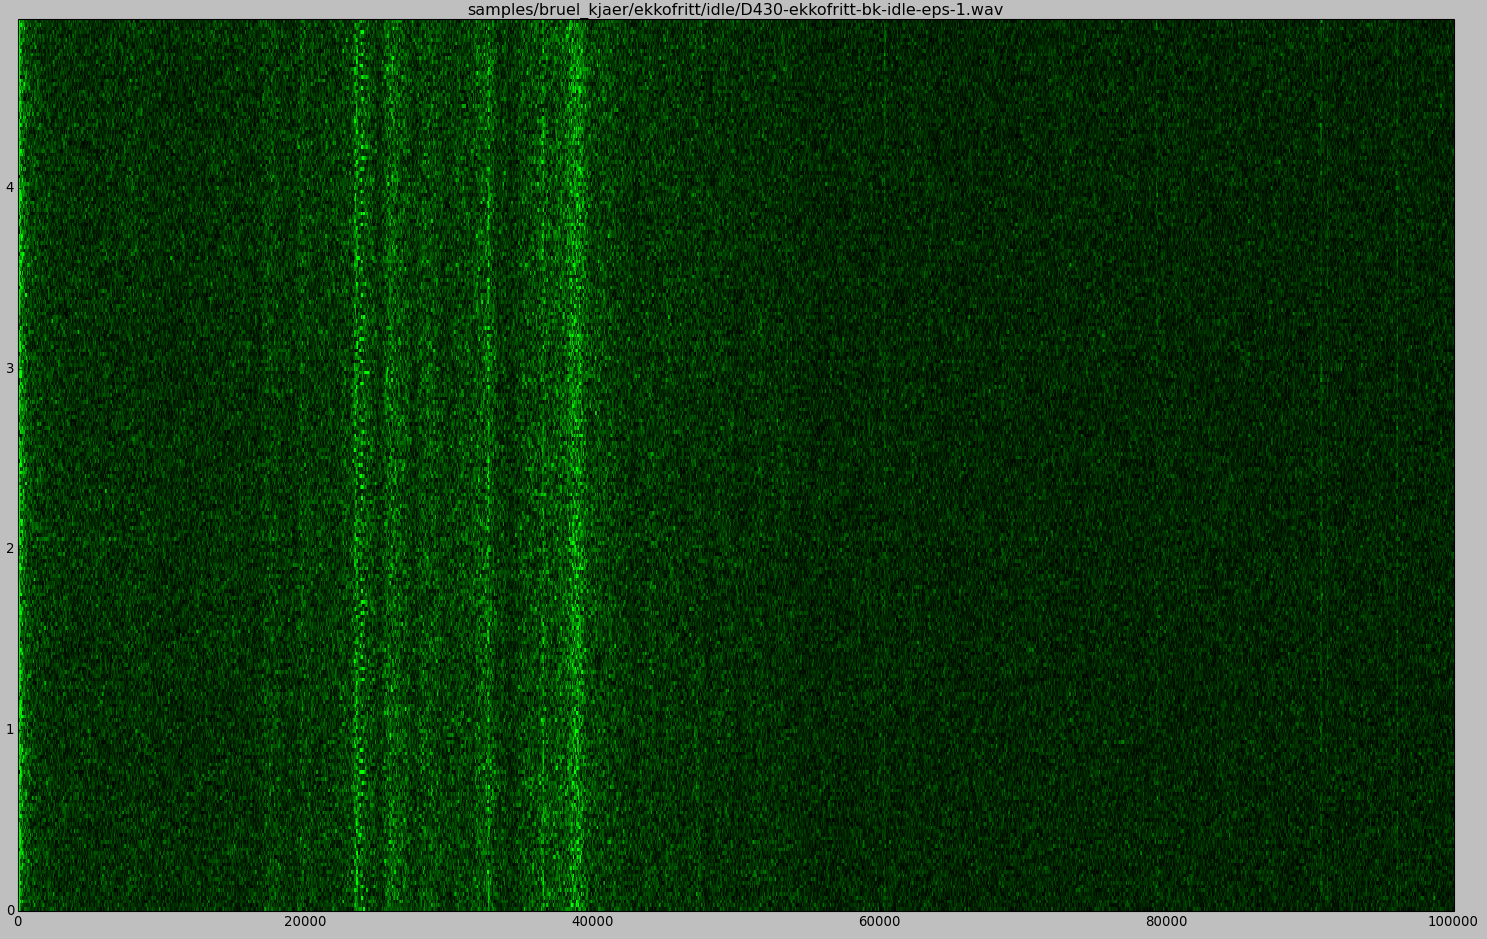
\includegraphics[width=1\linewidth]{D430-ekkofritt-bk-idle-eps-1.png}
    \caption{Acoustic recording (5 sec, 0-100kHz) of the Dell D430 when idle. The recording was made in an anechoic chamber using the Brüel\&Kjær 4939 microphone with the NI myDAQ. }
    \label{fig:D430-ekkofritt-bk-idle-eps-1}
\end{wrapfigure}


\begin{wrapfigure}{r}{1\textwidth}
	\begin{subfigure}{0.5\textwidth}
	    \centering
	    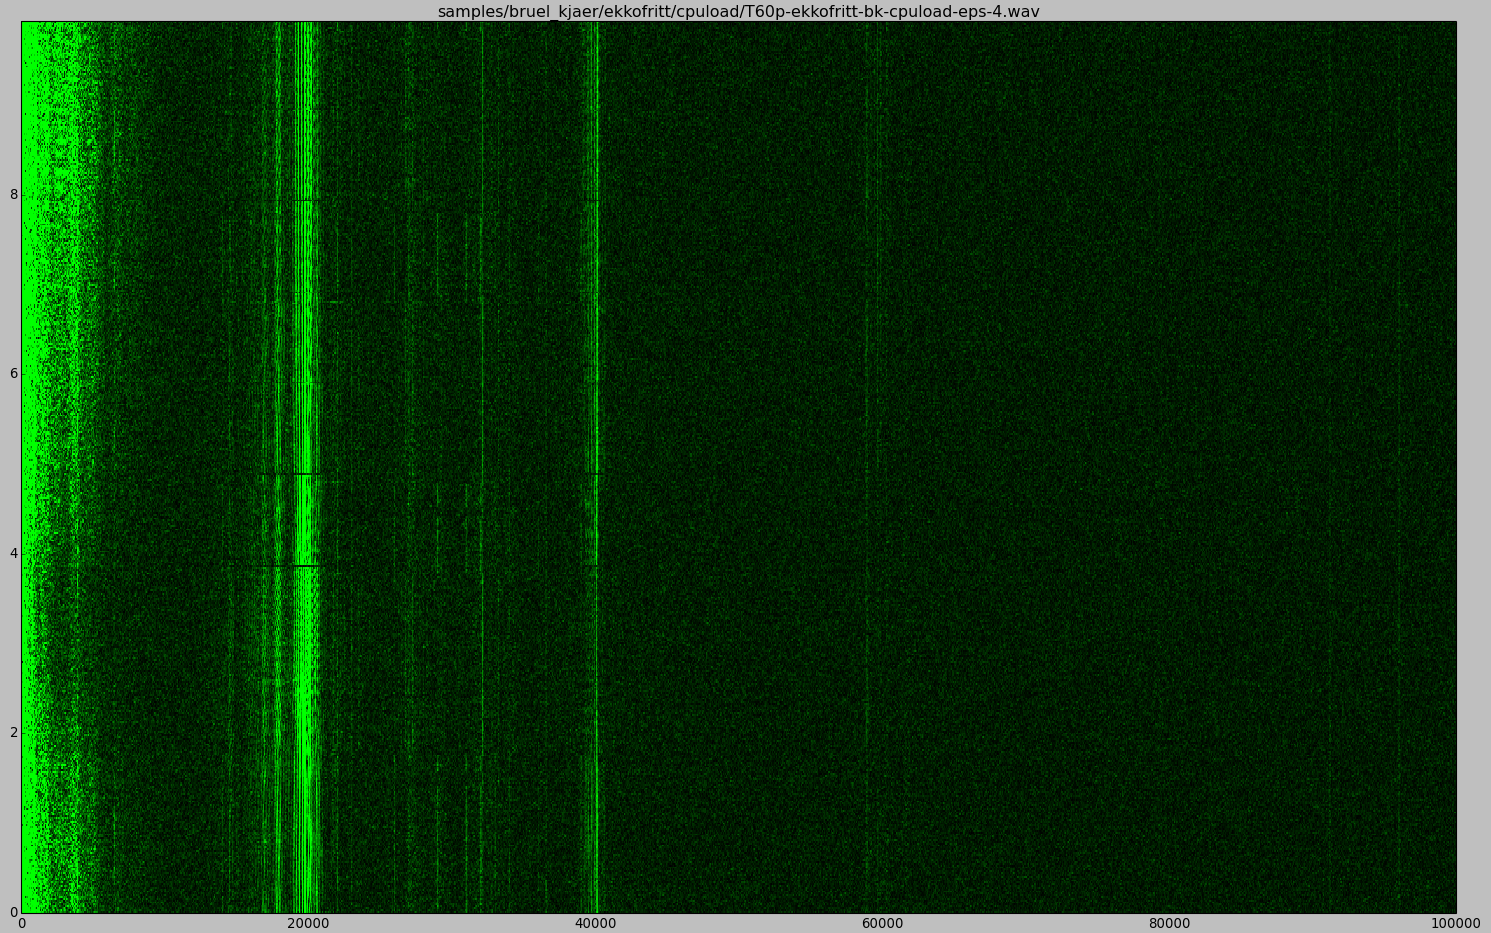
\includegraphics[width=1\linewidth]{T60p-ekkofritt-bk-cpuload-eps-4.png}
	    \caption{External power supply}
	    \label{fig:T60p-ekkofritt-bk-cpuload-eps-4}
    \end{subfigure}
    \begin{subfigure}{0.5\textwidth}
	    \centering
	    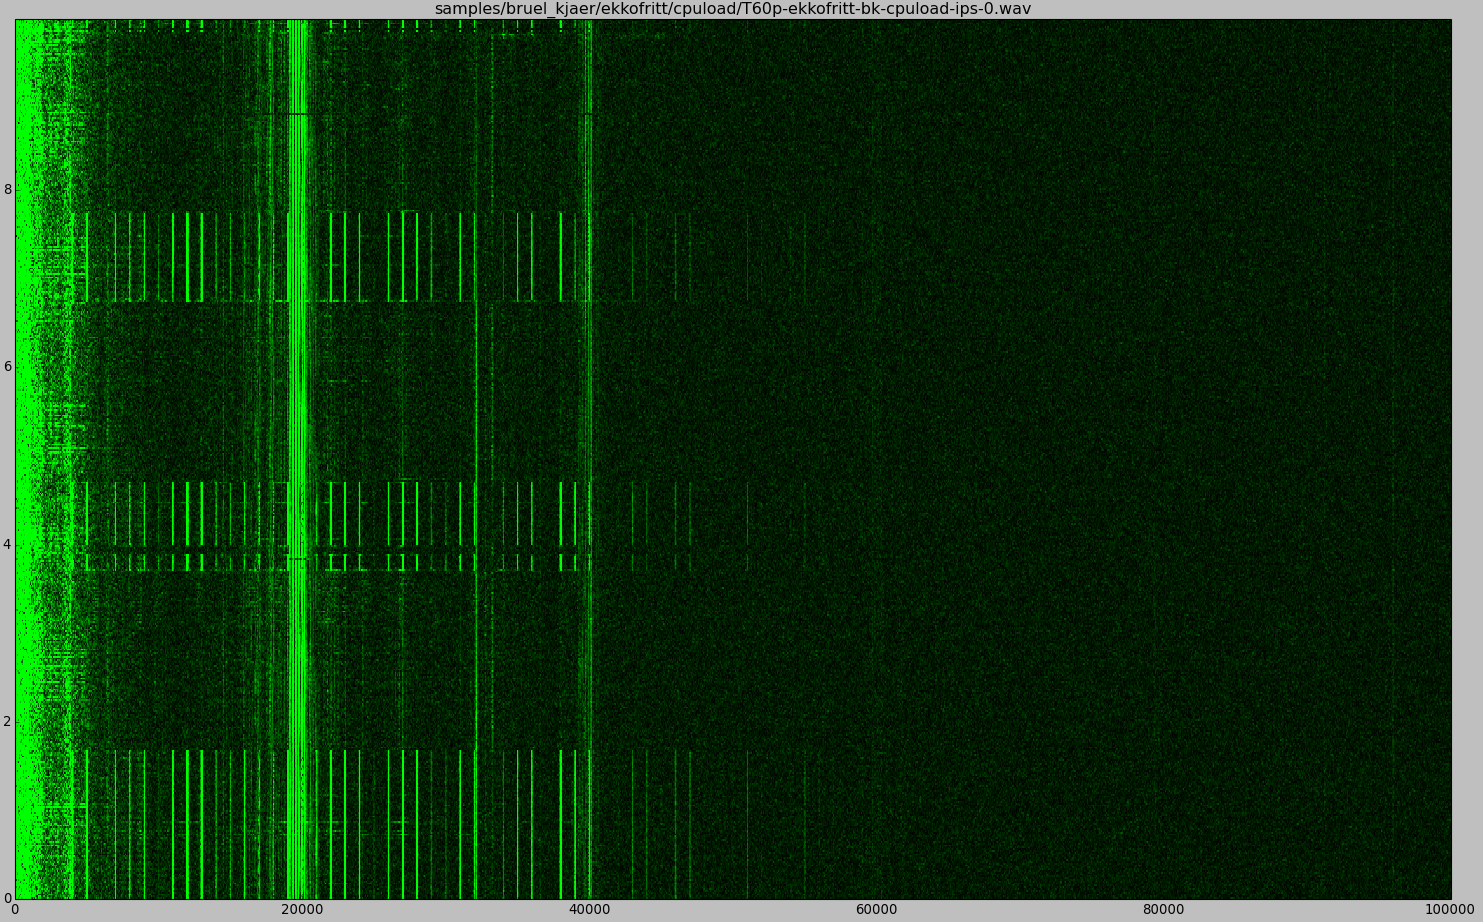
\includegraphics[width=1\linewidth]{T60p-ekkofritt-bk-cpuload-ips-0.png}
	    \caption{Internal power supply}
	    \label{fig:T60p-ekkofritt-bk-cpuload-ips-0}
    \end{subfigure}
    \caption{Acoustic recording (10 sec, 0-100kHz) of the Lenovo T60p when running a full CPU load. The recording was made in an anechoic chamber using the Brüel\&Kjær 4939 microphone with the NI myDAQ.}
	\label{fig:T60p-ekkofritt-bk-cpuload}
\end{wrapfigure}


\begin{wrapfigure}{r}{1\textwidth}
    \centering
    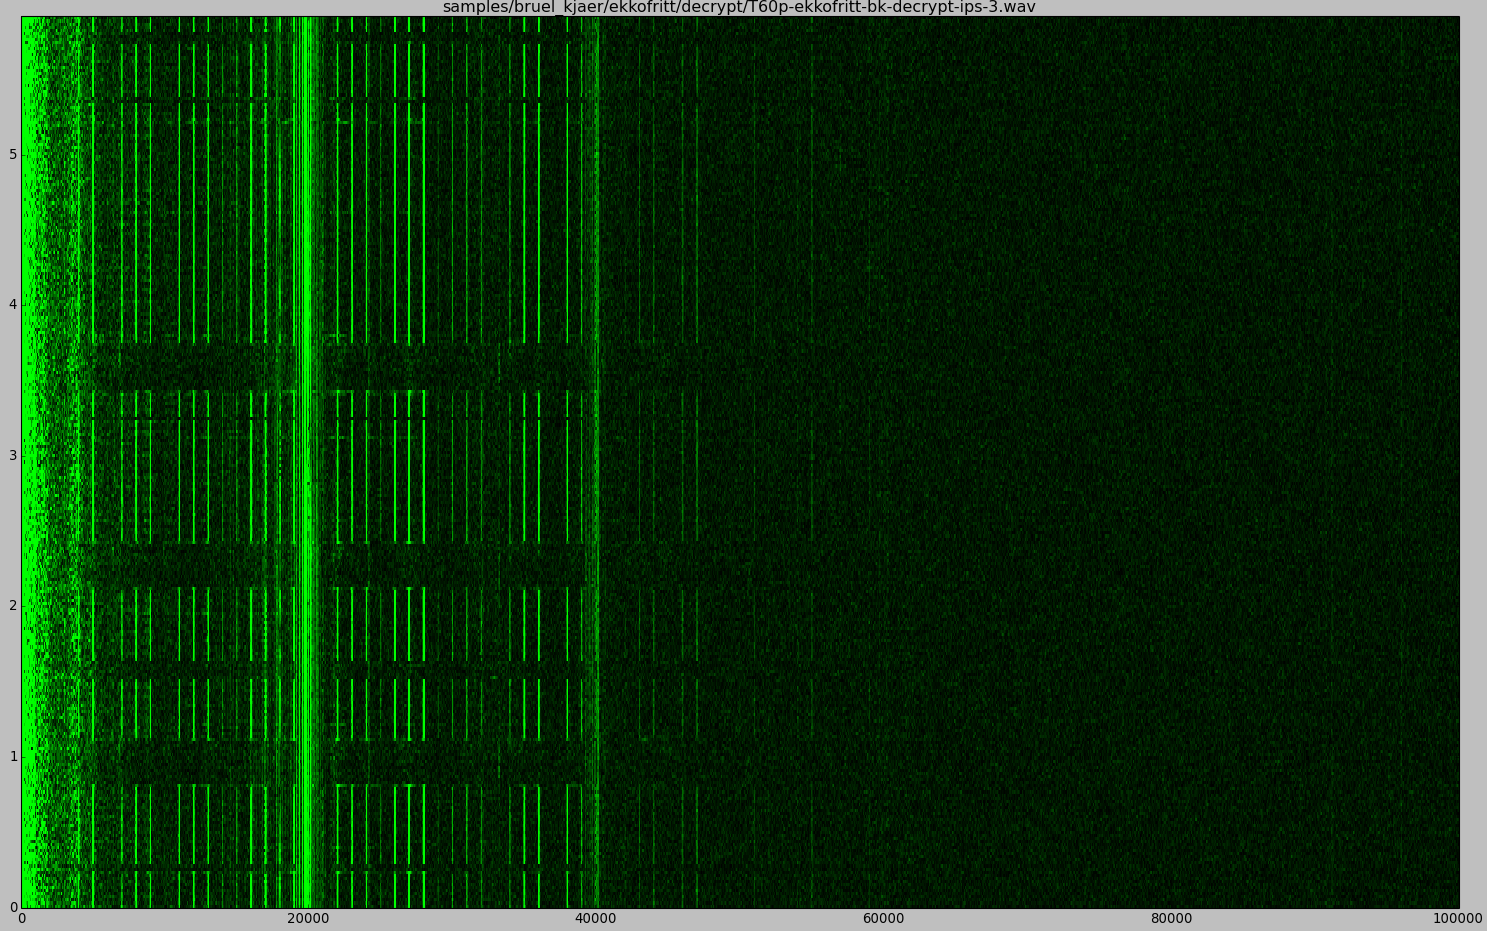
\includegraphics[width=1\linewidth]{T60p-ekkofritt-bk-decrypt-ips-3.png}
    \caption{Acoustic recording (6 sec, 0-100kHz) of the Lenovo T60p when running a dycrypt. The recording was made in an anechoic chamber using the Brüel\&Kjær 4939 microphone with the NI myDAQ. }
    \label{fig:T60p-ekkofritt-bk-decrypt-ips-3}
\end{wrapfigure}

\begin{wrapfigure}{r}{1\textwidth}
    \centering
    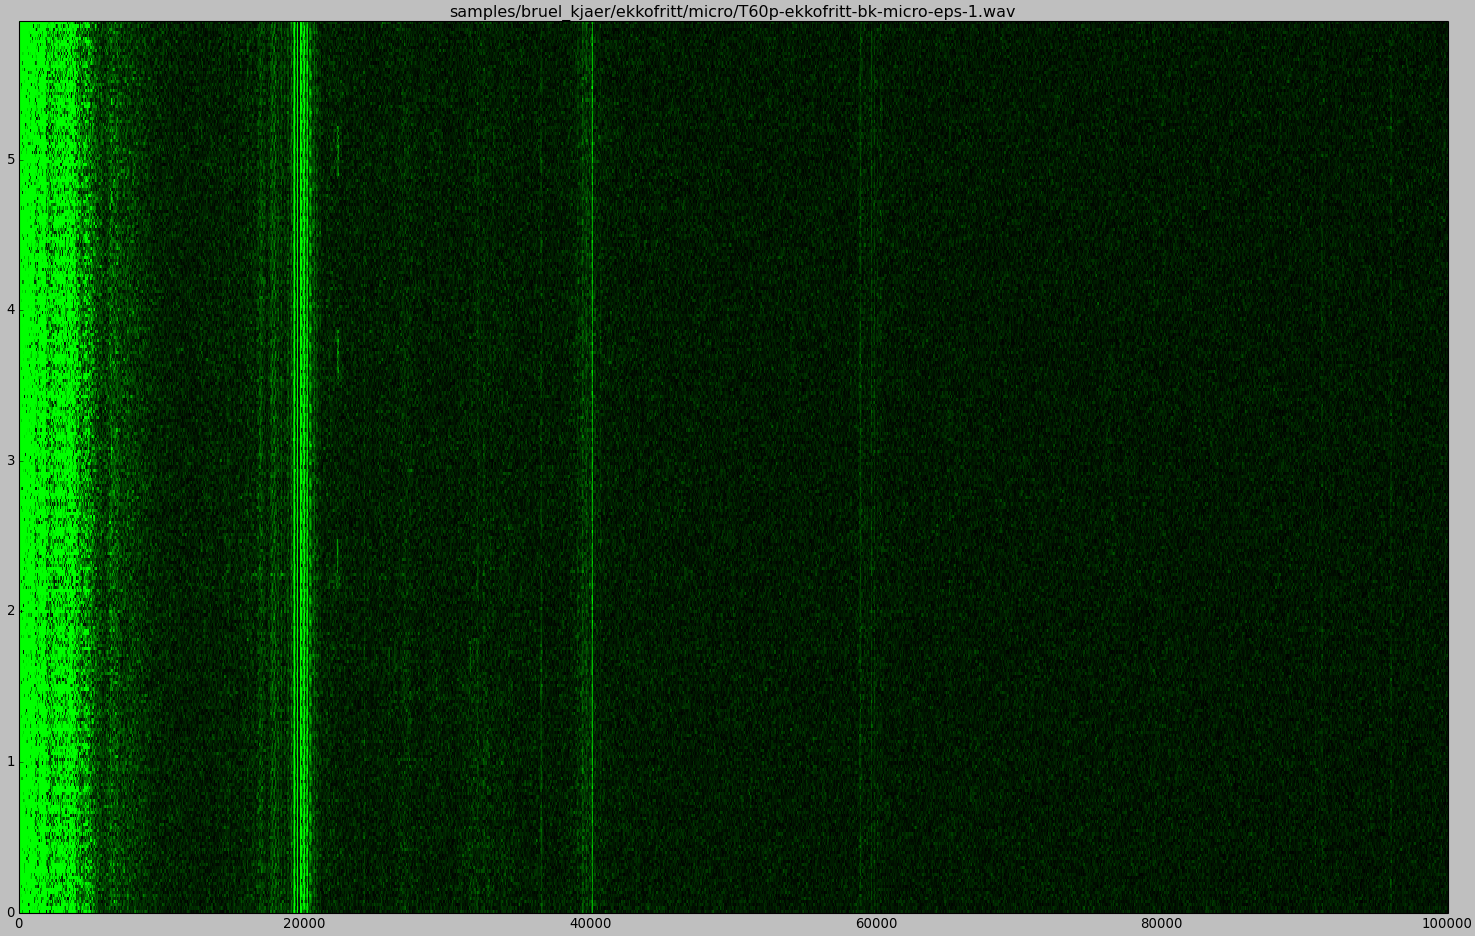
\includegraphics[width=1\linewidth]{T60p-ekkofritt-bk-micro-eps-1.png}
    \caption{Acoustic recording (6 sec, 0-100kHz) of the Lenovo T60p when running micro. The recording was made in an anechoic chamber using the Brüel\&Kjær 4939 microphone with the NI myDAQ. }
    \label{fig:T60p-ekkofritt-bk-micro-eps-1}
\end{wrapfigure}

\begin{wrapfigure}{r}{1\textwidth}
    \centering
    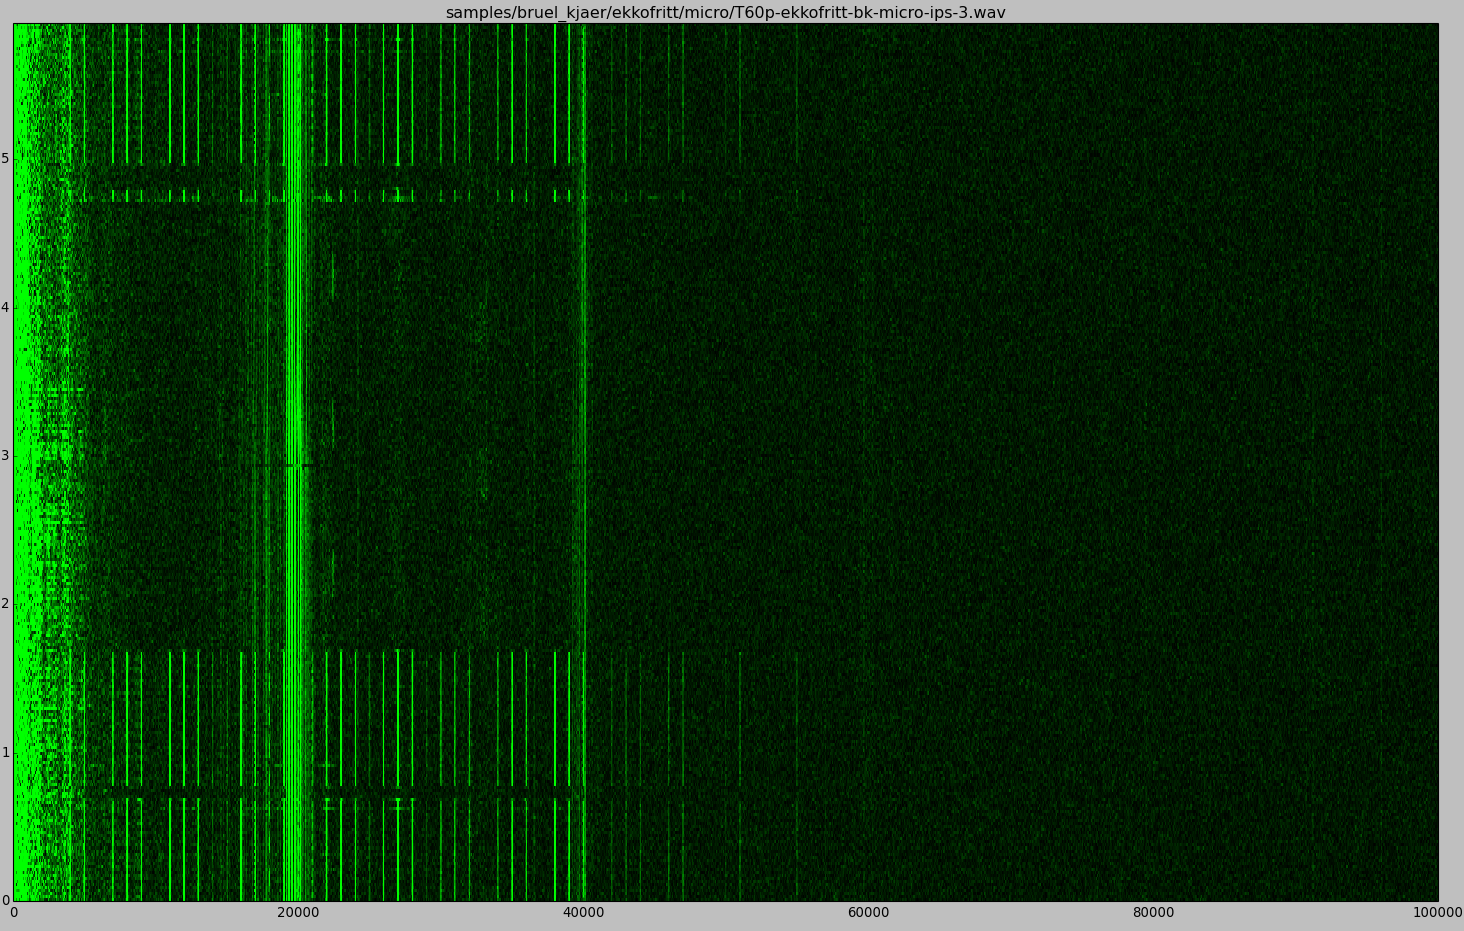
\includegraphics[width=1\linewidth]{T60p-ekkofritt-bk-micro-ips-3.png}
    \caption{Acoustic recording (6 sec, 0-100kHz) of the Lenovo T60p when running micro. The recording was made in an anechoic chamber using the Brüel\&Kjær 4939 microphone with the NI myDAQ. }
    \label{fig:T60p-ekkofritt-bk-micro-ips-3}
\end{wrapfigure}

\begin{wrapfigure}{r}{1\textwidth}
    \centering
    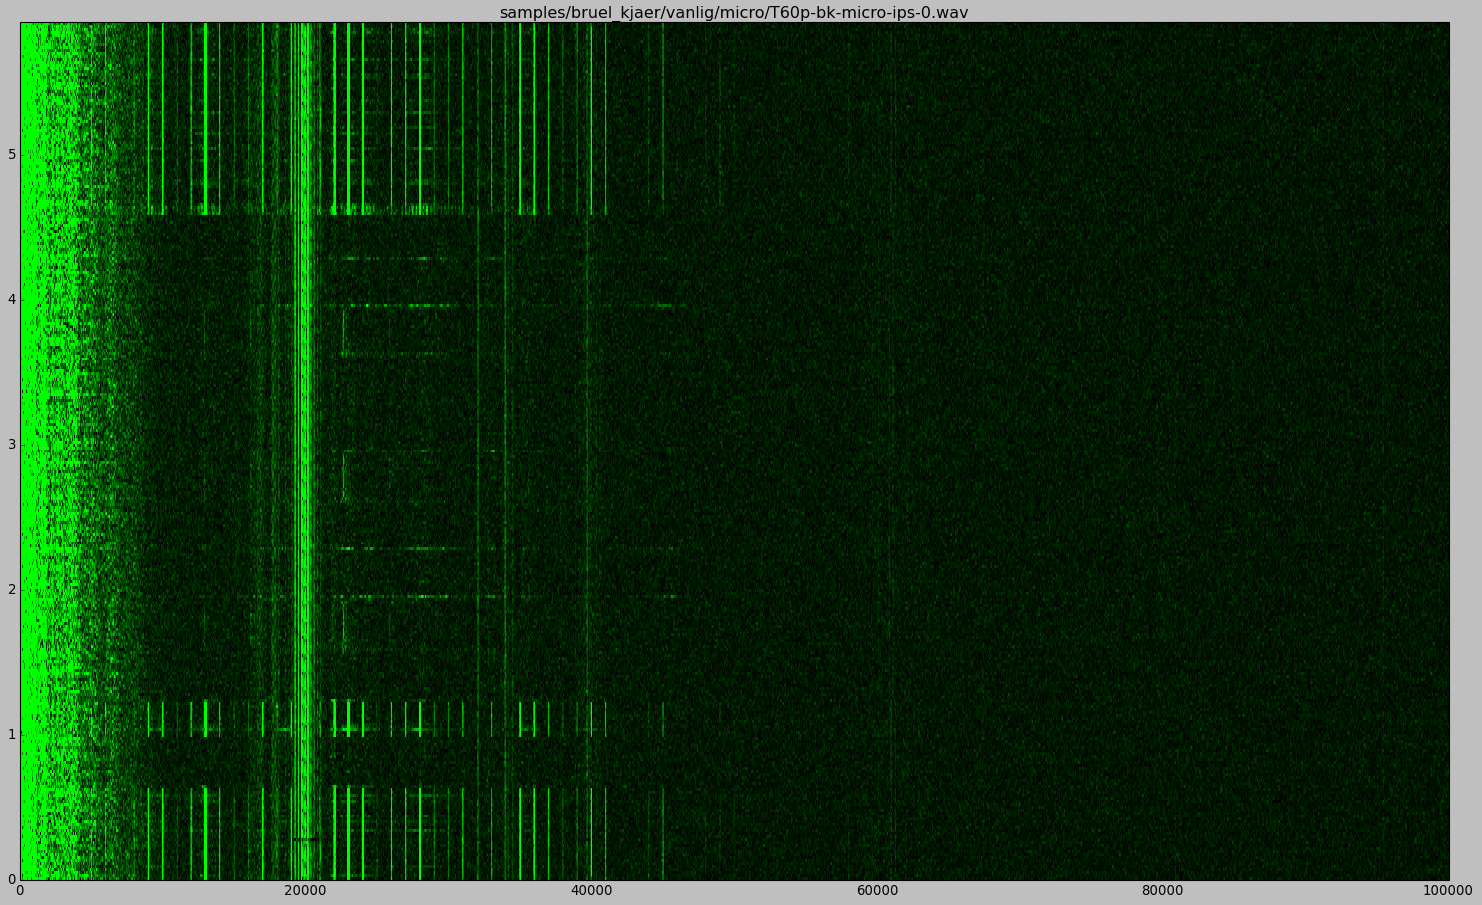
\includegraphics[width=1\linewidth]{T60p-bk-micro-ips-0.png}
    \caption{Acoustic recording (6 sec, 0-100kHz) of the Lenovo T60p when running micro. The recording was made using the Brüel\&Kjær 4939 microphone with the NI myDAQ. }
    \label{fig:T60p-bk-micro-ips-0}
\end{wrapfigure}

\begin{wrapfigure}{r}{1\textwidth}
	\begin{subfigure}{0.5\textwidth}
	    \centering
	    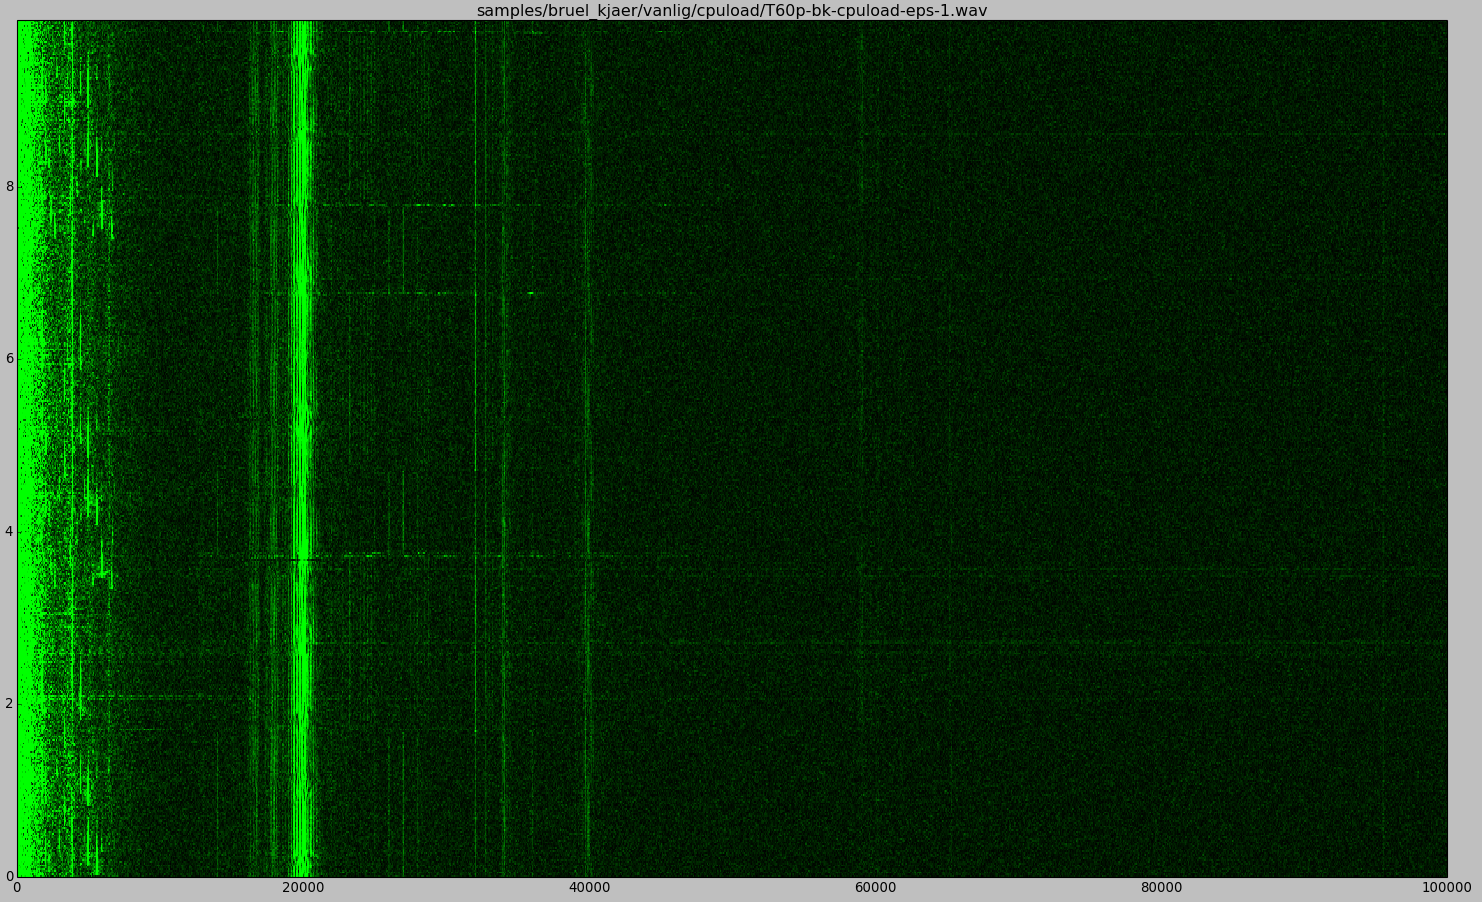
\includegraphics[width=1\linewidth]{T60p-bk-cpuload-eps-1.png}
	    \caption{External power suply}
	    \label{fig:T60p-bk-cpuload-eps-1-1a}
    \end{subfigure}
    \begin{subfigure}{0.5\textwidth}
	    \centering
	    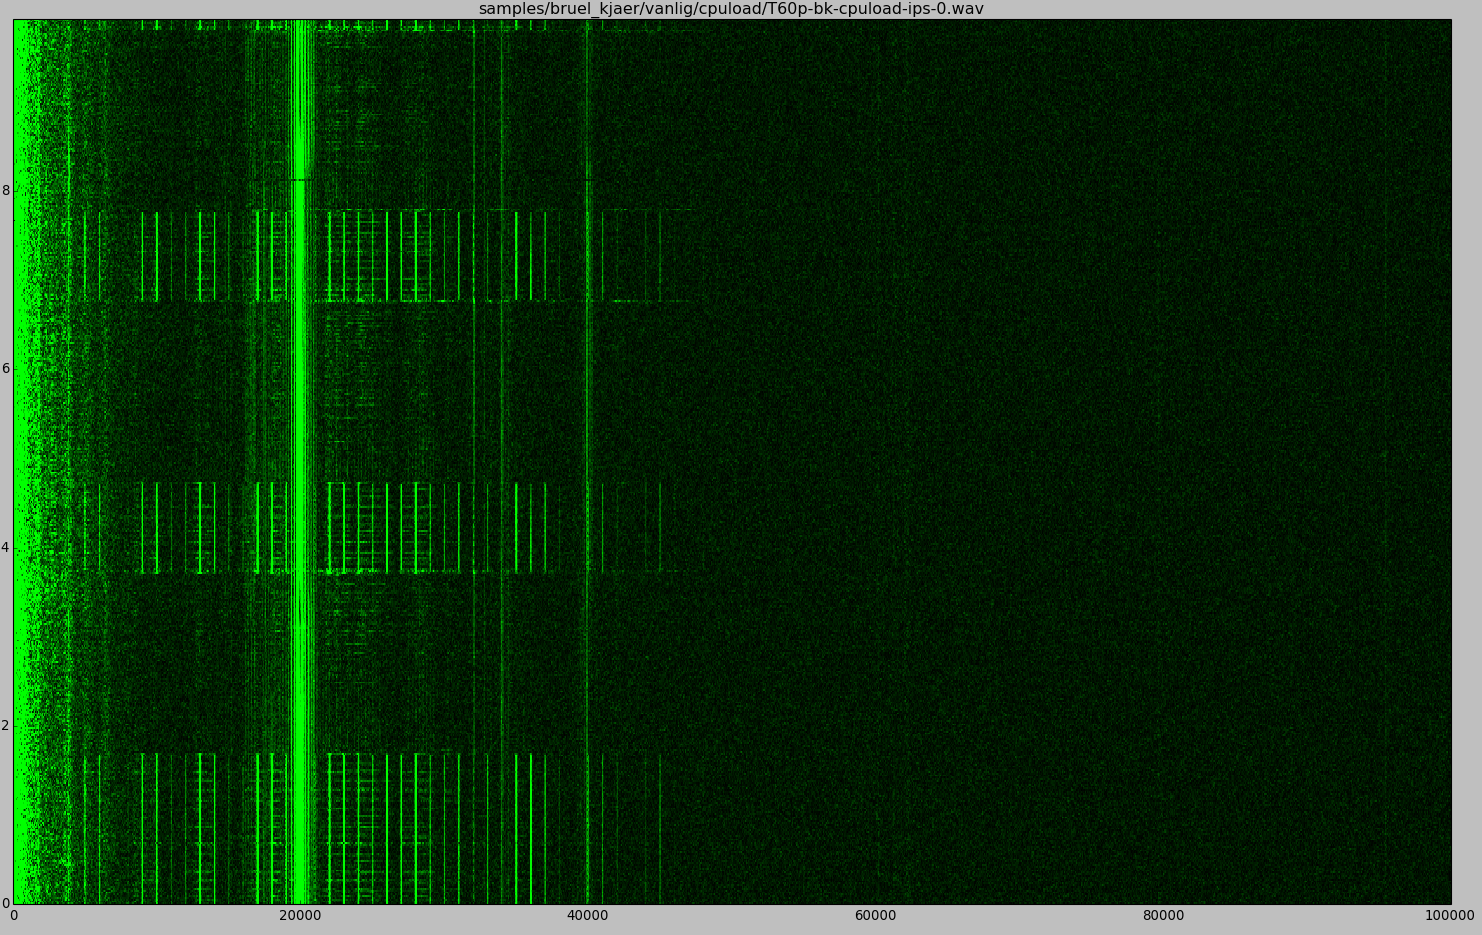
\includegraphics[width=1\linewidth]{T60p-bk-cpuload-ips-0.png}
	    \caption{Internal power suply}
	    \label{fig:T60p-bk-cpuload-ips-0-1b}
    \end{subfigure}
    \caption{Acoustic recording (10 sec, 0-100kHz) of the Lenovo T60p when running a full CPU load. The recordings was made using the Brüel\&Kjær 4939 microphone with the NI myDAQ. }
	\label{fig:T60p-bk-cpuload}
\end{wrapfigure}


\chapter{Discussion}\label{chp6:discussion}

In this chapter we will discuss the viability of the low frequency acoustic emanations, and how current guidelines for shielding information systems are helping in protecting against this potential threat.
We will also look at the cost involved in building a setup able to process these emanations, and the implications of this.
Last, we will look at use cases where the analysis of these emanations will be useful.

\section{Viability of Extracted Information}
We have not obtained a basis for drawing a conclusion as to whereas the emanations as presented in the previous chapters are in fact caused by the \gls{CPU}.
However, we have tried to capture the effect at different positions on our Lenovo T60p laptop. 
For this specific computer we experienced that it is far easier to find the patterns we are looking for in the resulting power spectra when the recordings are done right above the \gls{CPU}.
We also found that slight disposition of the microphone, still hovering the \gls{CPU} cooling block, notably impact the signal strength.


\section{Significance of Results}
Using the acoustic side channel, we are able to distinguish between the MEM operation and the other microinstruction loops.
The results given in~\cite[Fig.~2]{DBLP:conf/crypto/GenkinST14} suggest that it is possible to observe a difference, even between the different microinstructions ADD, MUL and NOP. 
The most visible difference is in a frequency range much higher than the hard limit imposed on us by the sampling rate of our setup.
Results given here are therefore inconclusive when it comes down to distinguishing between the NOP, MUL and ADD instructions.
~\autoref{fig:T60p-knowles-micro-ips-0}

We have conducted experiments using different configurations of hardware and observe big variations in acoustic fingerprints for the different computers, as seen in~\autoref{fig:comparison_micorinstructions}.
An interesting side note is how the acoustic emanations of the Lenovo T60p laptop is changing depending on if the computer is running on battery power (\autoref{fig:comparison_T60p-ekkofritt-bk-micro-ips-3}) or with a power adapter (\autoref{fig:comparison_T60p-ekkofritt-bk-micro-eps-1}).
The noise introduced by the power adapter is not emanating from the power adapter itself, as we have experimented with the positioning of the adapter, without seeing any impact on the resulting acoustic fingerprints.

We did not do any experiments to explore if the captured signals are in fact acoustic, or if they are caused by electromagnetic signals.

\begin{figure}[ht]
    \centering
    \begin{subfigure}{0.32\textwidth}
        \centering
        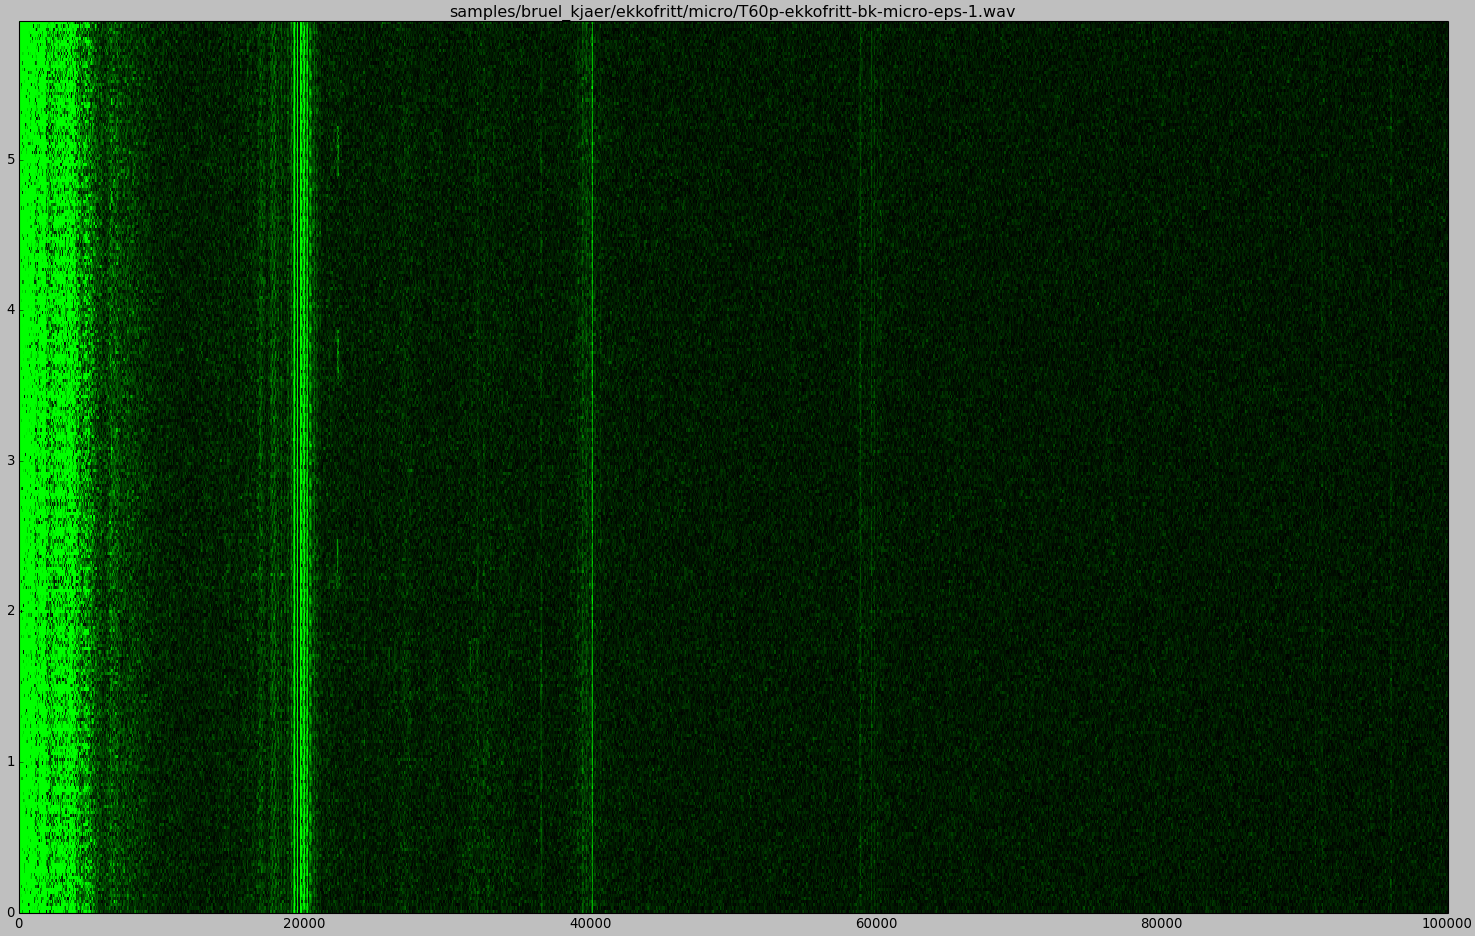
\includegraphics[width=1\linewidth]{T60p-ekkofritt-bk-micro-eps-1.png}
        \caption{Lenovo T60p}
        \label{fig:comparison_T60p-ekkofritt-bk-micro-eps-1}
    \end{subfigure}
    \begin{subfigure}{0.32\textwidth}
        \centering
        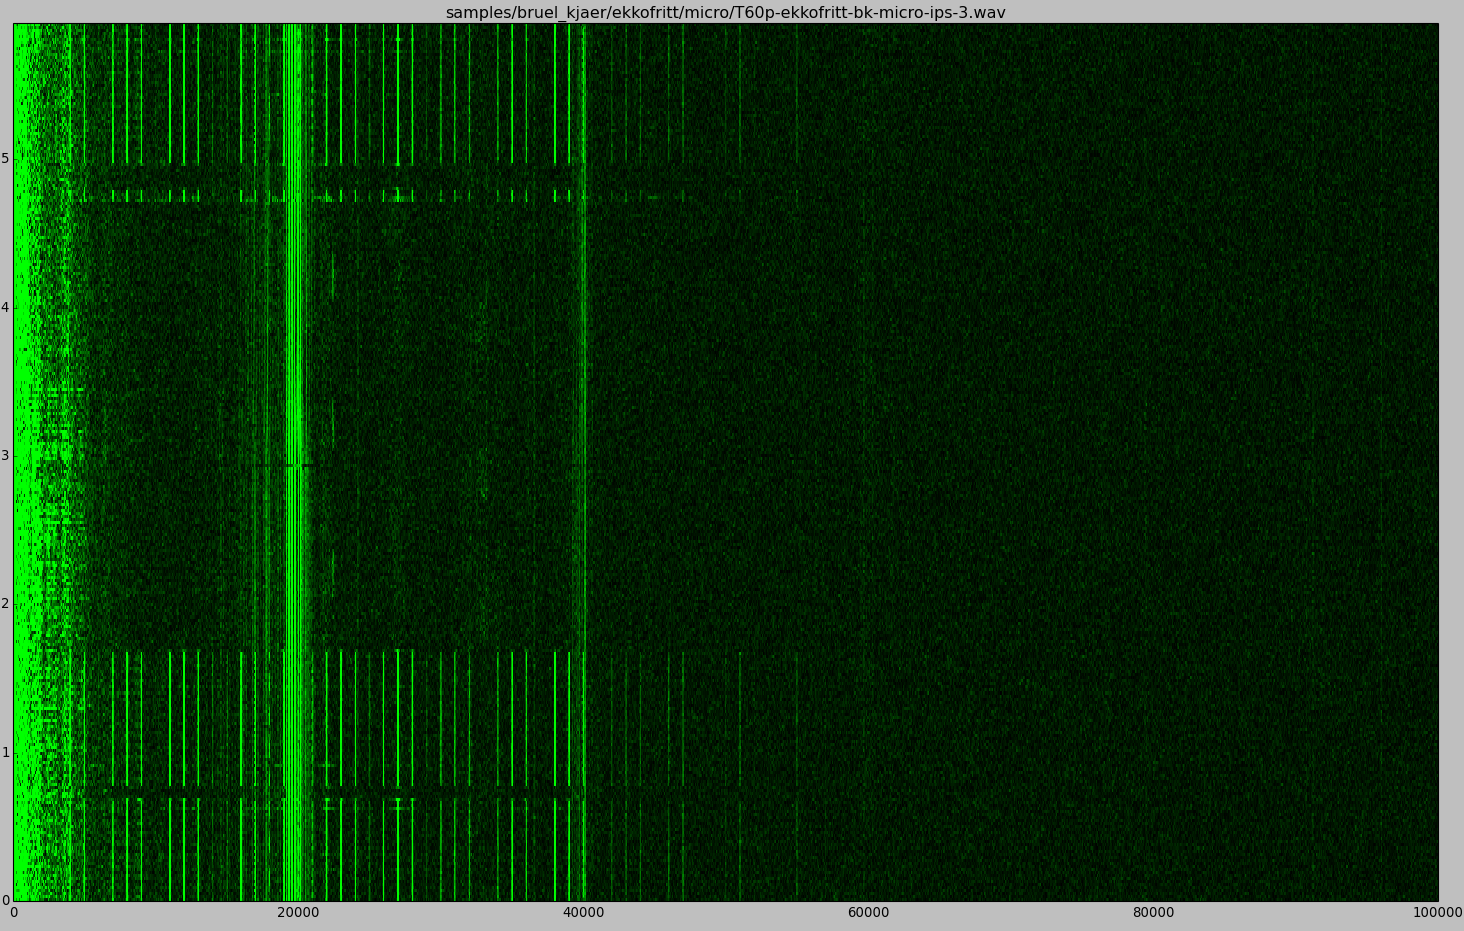
\includegraphics[width=1\linewidth]{T60p-ekkofritt-bk-micro-ips-3.png}
        \caption{Lenovo T60p}
        \label{fig:comparison_T60p-ekkofritt-bk-micro-ips-3}
    \end{subfigure}
    \begin{subfigure}{0.32\textwidth}
        \centering
        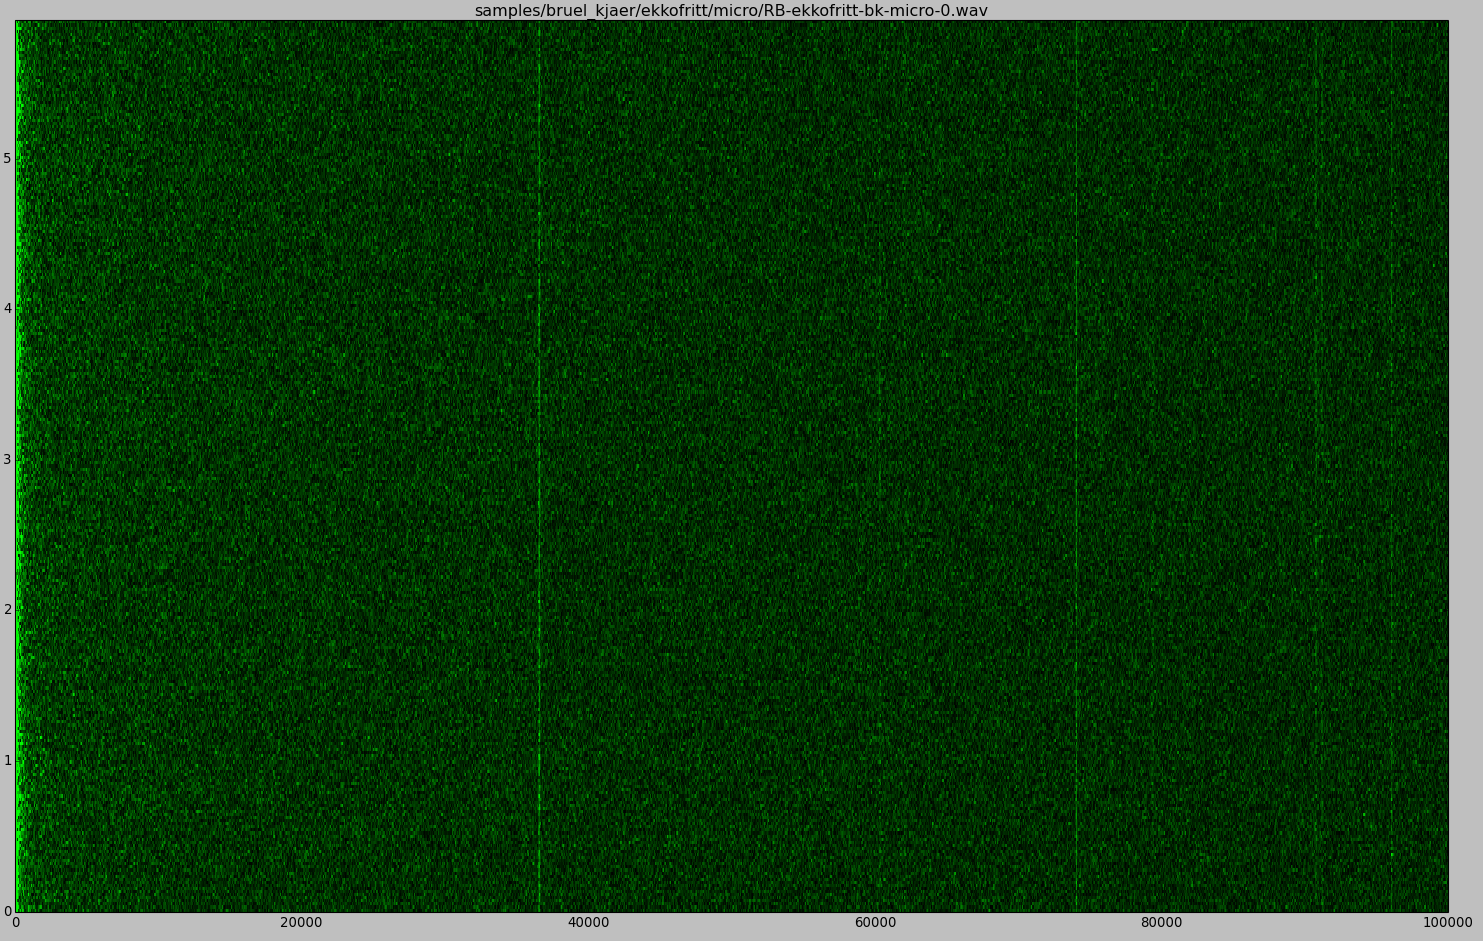
\includegraphics[width=1\linewidth]{RB-ekkofritt-bk-micro-0.png}
        \caption{Raspberry PI}
        \label{fig:comparison_RB-ekkofritt-bk-micro-0}
    \end{subfigure}
    \begin{subfigure}{0.32\textwidth}
        \centering
        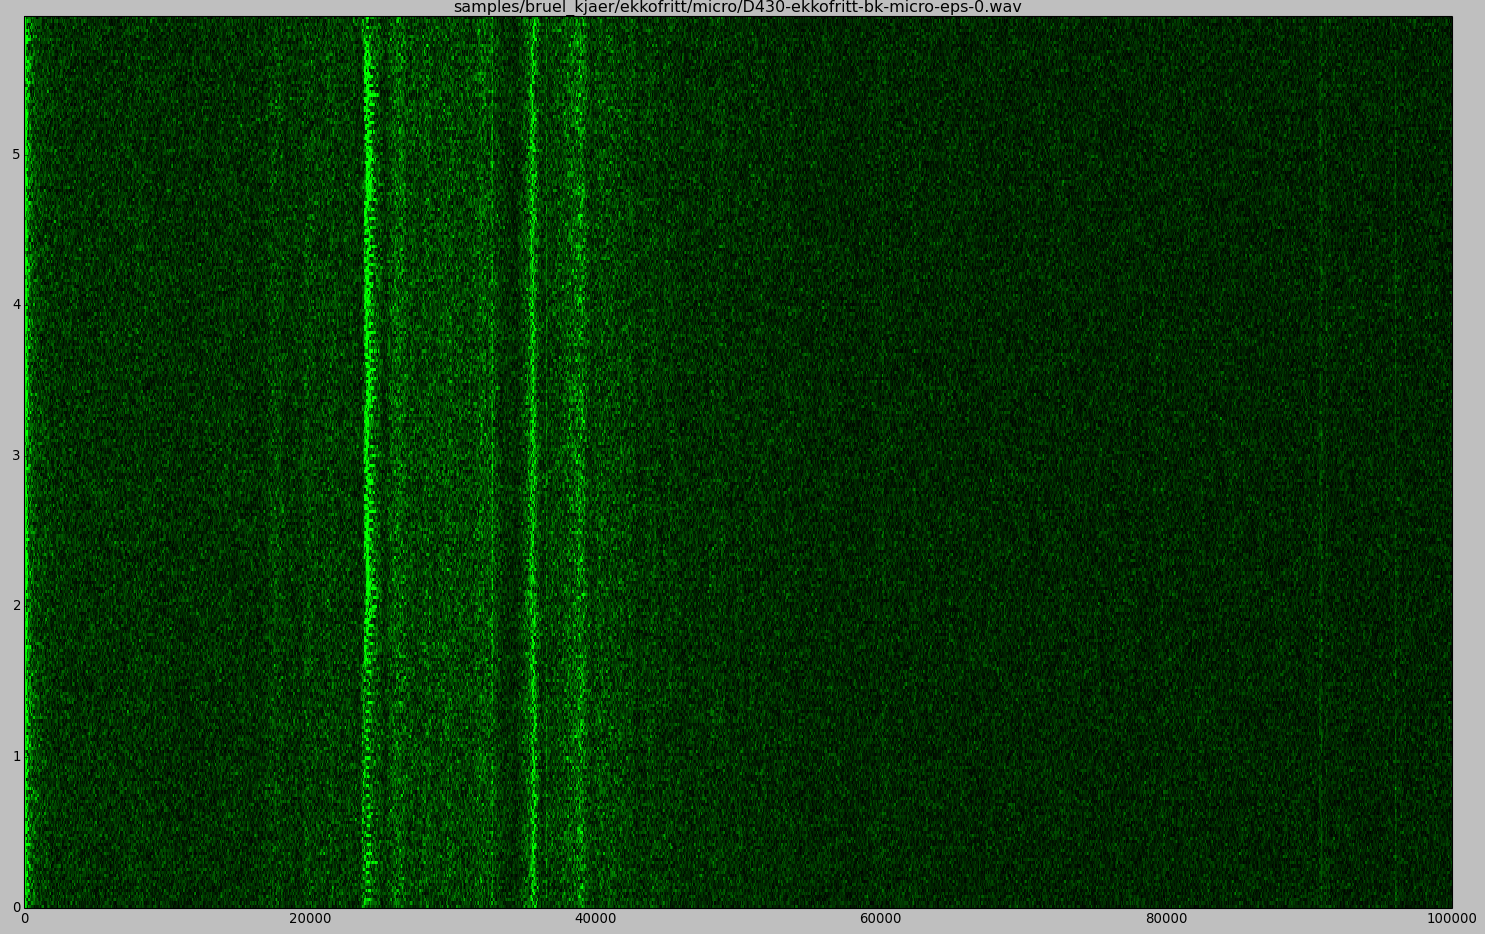
\includegraphics[width=1\linewidth]{D430-ekkofritt-bk-micro-eps-0.png}
        \caption{Dell 430}
        \label{fig:comparison_D430-ekkofritt-bk-micro-eps-0}
    \end{subfigure}
    \begin{subfigure}{0.32\textwidth}
        \centering
        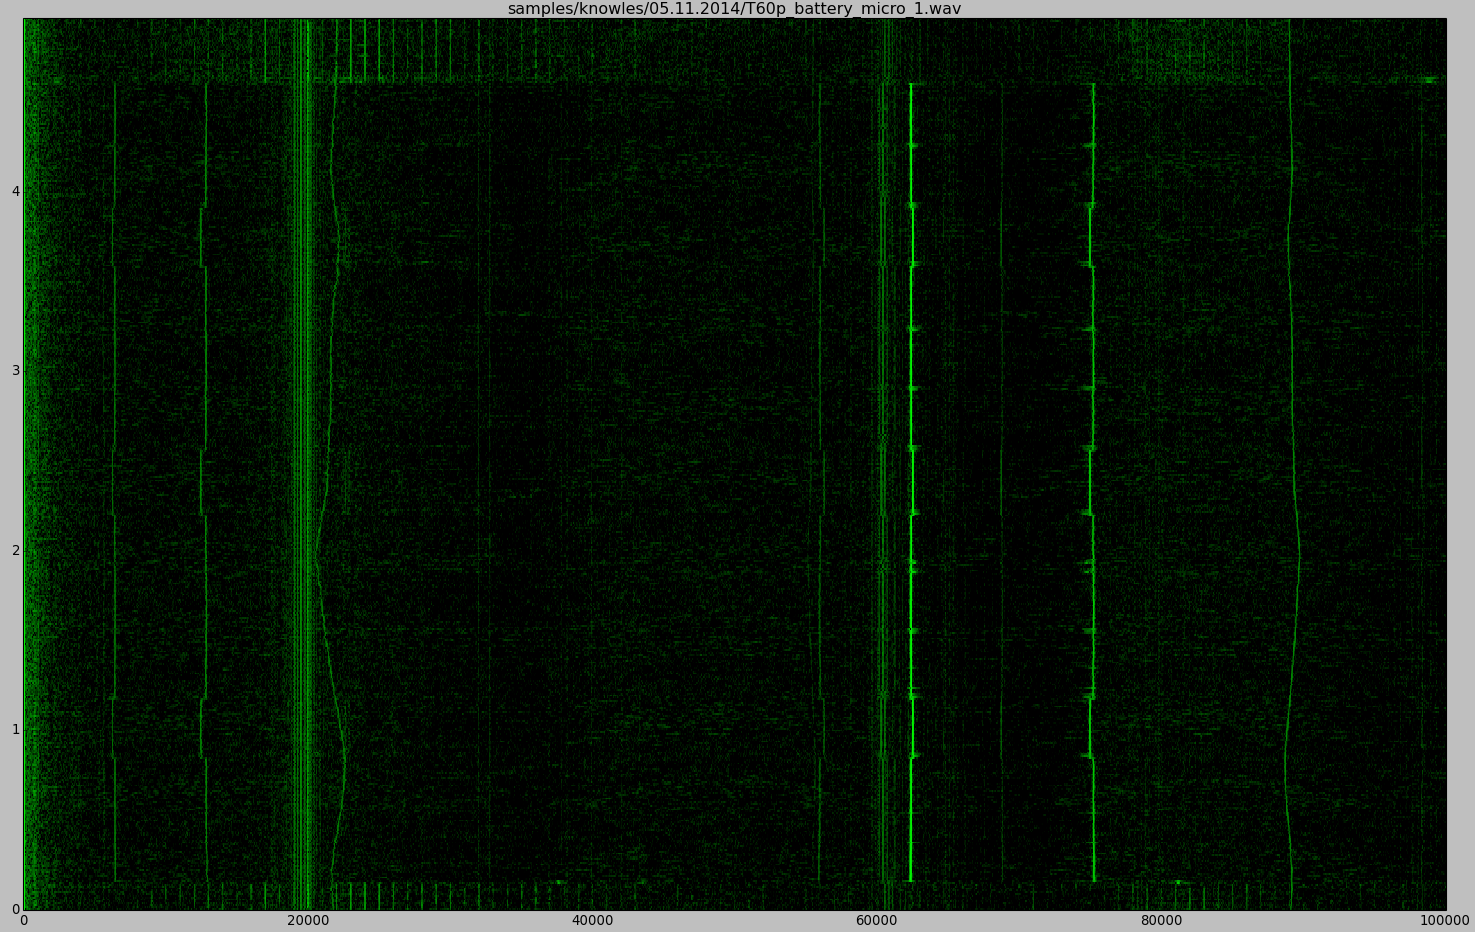
\includegraphics[width=1\linewidth]{T60p-knowles-micro-ips-0.png}
        \caption{Lenovo T60p}
        \label{fig:comparison_T60p-knowles-micro-ips-0}
    \end{subfigure}
    \begin{subfigure}{0.32\textwidth}
        \centering
        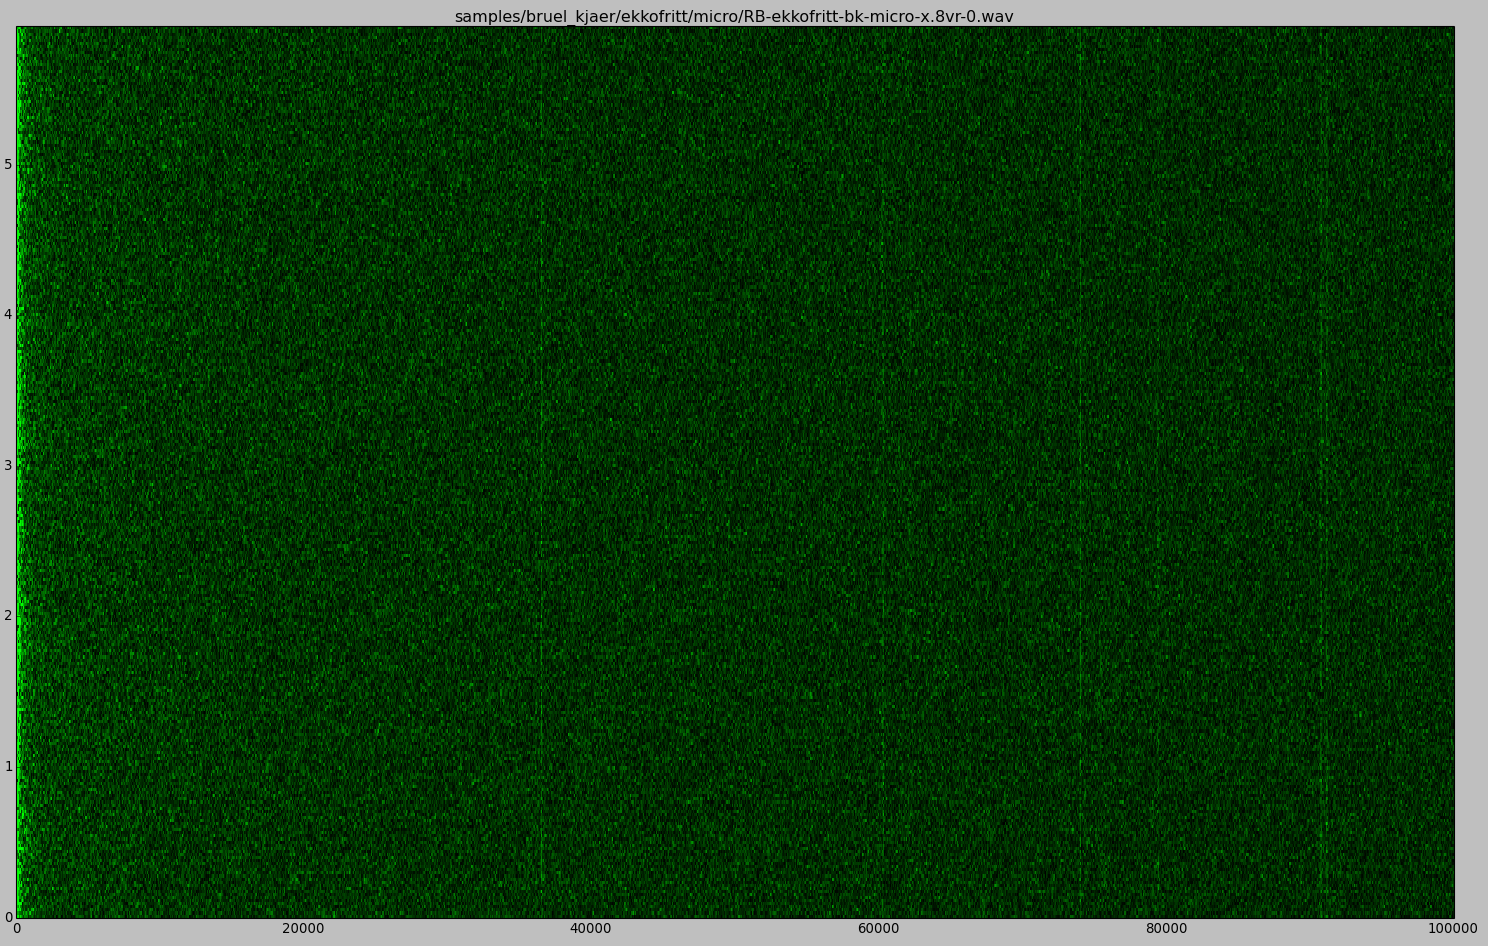
\includegraphics[width=1\linewidth]{RB-ekkofritt-bk-micro-x-8vr-0.png}
        \caption{Raspberry PI}
        \label{fig:comparison_RB-ekkofritt-bk-micro-x-8vr-0}
    \end{subfigure}
    \caption{ Acoustic emanations when performing the microinstructions on following devices:
    (a) T60p with Brüel\&Kjær running on power adopter.
    (b) T60p with Brüel\&Kjær running on battery power.
    (c) Raspberry PI on CPU with Brüel\&Kjær.
    (d) Dell D430 with Brüel\&Kjær running on battery power.
    (e) T60p with Knowles running on battery power.
    (f) Raspberry PI on power with Brüel\&Kjær.}
    \label{fig:comparison_micorinstructions}
\end{figure}

\section{Analysis Beyond Extremes}
In our experiments, we were able to distinguish between different extremes in \gls{CPU} activity based strictly on acoustic leakage. 
We do not use any mathematical models, but rely on empirical analysis of the power spectra. 
This is a limiting factor in the sense that we are only able to draw conclusions based on clear patterns in the resulting data that are visible to the human eye, when presented in the way done here and by Genkin et al.
None of the experiments we performed included real time analysis of the leakage, hence we were limited to look for patterns resulting from static programs being executed, to be able to relate the information captured to the time domain in our offline analysis.
Real time analysis, together with mathematical models for correlation, would allow a more statistical approach to distinguishing between distinct fingerprints, and could allow for attacks along the line of what is proposed in~\cite{DBLP:conf/crypto/KocherJJ99}, only using acoustic emanations rather than power traces for analysis.


\section{ARM Processors and Possible Attack Vectors}
We chose to conduct experiments on a Lenovo laptop computer similar to what is used by Genkin et al., and also on an even older Dell laptop, as it was suggested that older processors had more explicit acoustic fingerprints.
In addition, we conducted the same experiments for a Raspberry Pi, which is equipped with an ARM \gls{CPU}.

A motivation for looking at ARM processors is that a lot of electronic equipment today is running on the ARM architecture.
The potential of analyzing network traffic by looking at routers is just one of several interesting approaches to exploit the potential of low frequency acoustic emanations.
Unfortunately, we found it much harder to distinguish between operations on the Raspberry Pi, than for the laptops running on x86/x64 Intel processors.
It is still worth noting that the findings of Genkin et al. suggest that distinguishing between different RSA keys used for decryption can be done using this side channel; in the case of a router, this means that the approach could be a viable way to analyze ongoing IPSec sessions, where the router performs encryption or decryption, without being connected to the network at all.


\section{Possible Attack Scenarios}\label{chp6:sec:attack_scenarios}

Our portable setup (\autoref{chp3:sec:knowles_configuration}) could be made even smaller and mounted with a small transmitter. 
This makes the setup mountable on stationary computers, where it could be used for eavesdropping. 
\todo{write further}

Genkin et al. introduces some possible attack scenarios that could exploit the acoustic emanations in~\cite[Section 1.2 and Appendix B]{DBLP:journals/iacr/GenkinST13}

\section{Countermeasures}\label{chp6:sec:countermeasures}

In the guidance paper about protection against eavesdropping published by the \gls{NSM}, it is recommended that one should follow the TEMPEST guidance when installing an information system~\cite[Section 9.8, page 7]{url:NSM/avlytting}.
However, the shielding requirement for a TEMPEST certified equipment is made with respect to electromagnetic signals.
Thus TEMPEST requirements for shielding (e.g. a Faraday cage) might not enhance the protection against acoustic emanations. 

The Red/Black Engineering-Installation Guidelines~\cite[Section 30.1, page 91]{url:Red/Black/Engineering} created by the \gls{DoD}, states that unauthorized (BLACK) and authorized (RED) equipment should at least be separated with 3 feet / 0.9 meter. 
Other electronic devices such as mobile phones and personal laptops should not be permitted to areas where RED equipment is installed. 
Genkin et al. showed that they can recover a 4096-bit RSA key from 4 meters, in which 0.9 meter will not be sufficient distance depending on the acoustic signal strength. 

The strength of the acoustic signals we discovered is significantly high (audibly by the human ear) and will be hard to shield on a small laptop.
However, our observations enhances Genkin et al. suspicion of that the signal quality seems correlated to the computer's age, hence newer computers might be protected sufficiently. 


\chapter{Conclusion and Future Work}\label{chp7:conclusion}

\section{Conclusion}
In this paper we have conducted independent experiments with an aim on verifying the claims of Genkin et al. 
The experiments have touched a part of the results presented in~\cite{DBLP:conf/crypto/GenkinST14}, as they have aimed to verify the bare existence of the acoustic side channel as a viable medium to extract information leakage.

Our research show that we are able to support the claims that the acoustic side channel conveys enough information to distinguish between different low-level CPU operations.
We display that the \gls{SNR} in some cases is strong enough to easily spot such differences using simple plots of the frequency spectra.

The most significant result obtained is the clear display of difference in the acoustic fingerprint of the MEM operation and looping other microinstructions.
Differences can even be observed at frequencies in the audible range, which supports the claim made by Genkin et al., that a mobile phone's microphone can be used to extract viable information from the side channel.
Additionally, this suggests that low-cost equipment can be sufficient for information extraction over this side-channel, something which is supported by our results using our experimental recording setup as described in~\autoref{chp3:sec:knowles_configuration}.

Results presented in this paper support the claims by Genkin et al.; low-bandwidth acoustic emanations from computers carry information about the internal state of the \gls{CPU}.
Moreover, extracting this information can be done with a relatively cheap setup, under sub-optimal conditions.
Our experiments show that recording in an anechoic chamber is in no way a necessity, and that the \gls{SNR} while recording in a room full of other people and different computer equipment is sufficient to clearly see differences in the acoustic fingerprint of distinct \gls{CPU} operations.

\section{Future Work}\label{chp7:sec:future_work}
An assumption taken in our work is that the emanations observed during the experiments are in fact acoustic.
This question is discussed by Genkin et al., and they have conducted experiments to support their claim.
We have not reproduced any of these experiments, as we have merely looked at information leakage from CPUs operating under very specific conditions.
Future work should aim to support the theory that the emanations are indeed acoustic.
Additionally, understanding the phenomenons causing the emanations, and identifying the source should be subject to future research.


\begin{enumerate}
	\item ADD loops of different lengths
	\item Statistical models for correlation
	\item Real time analysis
	\item Experiments on the proposed attack against RSA
	\item Listening to GPU for reproducing display
\end{enumerate}

%% include here the other chapters

%% References
%\renewcommand*{\bibname}{References}
\bibliographystyle{plain}
\bibliography{references}

\begin{thebibliography}{11}

%========================
% Original Paper Research
%========================

\bibitem{original_paper} Tromer, et al: RSA Key Extraction via Low-Bandwidth Acoustic Cryptanalysis. Tel Aviv 2014 
\url{http://cs.tau.ac.il/~tromer/acoustic/}


%===================================
% Background: Acoustic cryptanalysis
%===================================

\bibitem{keystrokes} Researchers recover typed text using audio recording of keystrokes. Date visited: 9.oct 2014, 
\url{http://www.berkeley.edu/news/media/releases/2005/09/14_key.shtml}

\bibitem{KybdEmanation} Dmitri Asonov and Rakesh Agrawal. Keyboard Acoustic Emanations. San Jose 2004
\url{http://www.davidsalomon.name/CompSec/auxiliary/KybdEmanation.pdf}

%===========================
% Background: Data remanence
%===========================

\bibitem{data_remanence_flash} Sergei Skorobogatov. Data Remanence in Flash Memory Devices. United Kingdom 2005. 
\url{https://www.cl.cam.ac.uk/~sps32/DataRem_CHES2005.pdf}

%========================================
% Background: Differential fault analysis
%========================================

\bibitem{dfa_guo} Guo, et al. Invariance-based concurrent error detection for advanced encryption standard. New York 2012.
\url{http://dl.acm.org/citation.cfm?id=2228463}

\bibitem{dfa_aes} Giraud (2003): DFA on AES
\url{http://citeseerx.ist.psu.edu/viewdoc/summary?doi=10.1.1.12.1030}

%====================================
% Background: Electromagnetic attacks
%====================================

\bibitem{tempest_sans} SANS Institue. An Introduction to TEMPEST
\url{http://www.sans.org/reading-room/whitepapers/privacy/introduction-tempest-981}


%===========================
% Background: Power analysis
%===========================

\bibitem{dpa_kocher} Paul Kocher. Differential power analysis. San Francisco 1999.
\url{http://www.cryptography.com/public/pdf/DPA.pdf}

%===========================
% Background: Timing attacks
%===========================

\bibitem{ssl_timing_attack} D. Boneh and D. Brumley. Remote timing attacks are practical
\url{http://crypto.stanford.edu/~dabo/abstracts/ssl-timing.html}

\bibitem{timing_attack_kocher} Paul Kocher. Timing attacks on implementations of Diffie-Hellman, RSA, DSS and other systems. San Francisco 1996.
\url{http://www.cryptography.com/public/pdf/TimingAttacks.pdf}

%=============================================
% Knowles Ultrasonic SPU0410LR5H Configuration
%=============================================

\bibitem{knowles_spec} Knowles Ultrasonic SPU0410LR5H specification
\url{http://www.knowles.com/eng/content/download/4015/50958/version/4/file/SPU0410LR5H.pdf}

\end{thebibliography}
\renewcommand*{\bibname}{References}
\bibliographystyle{ieeetr}
%\bibliographystyle{alpha}
\bibliography{main}

% Uncomment the following if you have any appendix
\appendix
\addtocontents{toc}{%
 \protect\vspace{1em}%
 \protect\noindent \bfseries \appendixtocname\protect\par
 \protect\vspace{-.5em}%
}
\renewcommand{\chaptername}{\appendixname}
% include below possible appendices (chapters)
\chapter{Experiment Plan}\label{apx:experiment_plan}
This appendix will present our experiment plan, and the planning done prior to the execution of the recording experiments.

\section{Requirements}

We will perform recordings on the following target computers, prepared with programs tailored for this experiment\footnote{The computers are running all our utilities, as described in \autoref{chp:predictable_execution}}.
\begin{description}
	\item[Lenovo Thinkpad T60p] The casing will be partially removed, to allow for recordings closer to the CPU. We will experiment with the distances $0.5$ cm and $30$ cm from the CPU, and we will record while the computer is running both with a power adapter, and on battery power. All permutations of these two parameters add up to four configurations for us to experiment with.
	\item[Dell Latitude D430] For this computer we will record through the CPU fan exhaust, at an approximate distance from the CPU of $2$ cm.
	\item[Raspberry Pi model B] We will record with emphasis on three different positions: the CPU, the $3.3V$ regulator, and the area around the $1.8V$ and $2.8V$ regulators\footnote{The Raspberry Pi model B layout is described in this figure \url{http://upload.wikimedia.org/wikipedia/commons/a/af/Raspberrypi_pcb_overview_v04.svg} (Accessed 17-Nov 2014)}.
\end{description}

Further we will use the following equipment:
\begin{description}
	\item[Microphone] Brüel \& Kjær 4939
	\item[Preamplifier] Norsonic 1201
	\item[Amplifier] Norsonic type 336 (S/N 20626)
	\item[Filter] Krohn-Hite Corporation Model 3945 (S/N 005133)
	\item[Configuration] Ribbon Tweeter Banddiskant D8C, Kenwood FG-275 Function Generator.
	\item[Miscellaneous] Power chords, Camera for documentation, notebook
\end{description}

All recordings will be done twice: in an office environment, with unpredictable sources of background noise; and in an anechoic chamber, with minimal levels of background noise.

\section{Experiments}

The following experiments will be performed on all of the target computers, for all configurations, as given in the previous section.
Everything will take place first in the office environment, and then repeated in the anechoic chamber. The following cases are recorded in this order for the three computers, with all the configurations listed\footnote{All recordings are repeated five times to help distinguish between phenomenons caused by chance, and actual phenomenons caused by the activity we force on the CPU.}.

\begin{enumerate}
	\item A reference recording of a sinusoid produced by the Ribbon Tweeter and the Function Generator, to verify that our setup is in fact recording and working as intended.
	\item Reference recordings of the target computer in idle state for $5$ seconds.
	\item Recordings of the CPU load, running the code described in \autoref{chp4:cpu_load}.
	\item Recordings of different microinstructions, running the microinstruction loop described in \autoref{chp4:microinstructions}.
	\item Recordings of the computer doing decryption, as described in \autoref{chp4:decryption}. 
\end{enumerate}
\chapter{Code Used in Analysis}\label{apx:code}

\section{Processing Sound Files}
The following program written in C was used to process the sound files recorded in our experiments. 
The reason for writing the program this way is because we were more comfortable with writing in C than using i.e. Matlab.
Additionally, we think this code is very adoptable, and can easily be adjusted to process real time recordings.

\section{Usage}
The output from \autoref{lst:main.c} is piped to \autoref{lst:plot.py}, to produce a plot representing the frequency response for the duration of the recording. 


\section{Signal Processing in C}
The signal processing is done with \autoref{lst:main.c}, a routine written in C.
The frequency responses resulting from each Fourier transformed window is passed to the standard output, as well as some meta data.

\begin{lstinputlisting}[language=C, caption={main.c - Compute Power Spectrum of a Sound File}, label={lst:main.c}]{code/main.c}
\end{lstinputlisting}


\section{Plotting in Python}
Plotting is done using the Python script given in \autoref{lst:plot.py}.
The data is read from standard input, i.e. the output from the signal processing routine.
Simple operations, such as applying a logarithmic scale to the spectra, and setting thresholds for the plot is done by tuning parameters in this script.

\begin{lstinputlisting}[language=Python, caption={plot.py - Plot frequency spectra on time axis}, label={lst:plot.py}]{code/plot.py}
\end{lstinputlisting}

\chapter{MEM Operation Benchmark}\label{apx:mem_benchmark}

\section{Forcing Cache Misses}

The cache misses making up the MEM operation, as explained in \autoref{chp4:subsec:MEM_operation}, were generated by running the code given in \autoref{lst:1k_cache_miss.c} in a time-bound loop.
Benchmarking the code, to verify the ability to forced increased amount of  suffered cache misses, was done by comparing the results of running this code with the results from the code given in \autoref{lst:1k_cache_hit.c}.
These two pieces of code only differ on one single line, namely line number $22$, where in \autoref{lst:1k_cache_miss.c} the random number is used for lookup, while in \autoref{lst:1k_cache_hit.c} the deterministic iteration counter is used.

\begin{lstinputlisting}[language=C, caption={1k\_cache\_miss.c - Force 1000 cache misses}, label={lst:1k_cache_miss.c}]{code/cachemiss.c}
\end{lstinputlisting}

\begin{lstinputlisting}[language=C, caption={1k\_cache\_hit.c - Cache miss reference}, label={lst:1k_cache_hit.c}]{code/cachehit.c}
\end{lstinputlisting}

\section{Collecting Results}

The data behind \autoref{fig:mem_benchmark} were generated by running the Python script given in \autoref{lst:benchmark_cache_misses.py} on both the target laptops.

\begin{lstinputlisting}[language=Python, caption={benchmark\_cache\_misses.py - Collect data from 1000 runs of the forced cache miss and reference benchmark utilities.}, label={lst:benchmark_cache_misses.py}]{code/benchmark_cache_misses.py}
\end{lstinputlisting}

\chapter{Miscellaneous Results}\label{apx:results}
This appendix will present miscellaneous results not presented in the paper.
All executions presented in the results in this section are described in~\autoref{chp4:predictable_execution} unless else specified. 
Generally we have three different executions; CPU operations described in~\autoref{chp4:sec:microinstructions}, CPU load described in~\autoref{chp4:sec:cpu_load} and decryption described in~\autoref{chp4:sec:decryption}. 
We are working with two different microphone configurations, the portable setup and the lab grade setup, which is explained more in detail respectively in~\autoref{chp3:sec:knowles_configuration} and~\autoref{chp3:sec:bruel_kjaer_configuration}.

\section{Normal office environment}

%==========================
% T60p Normal room CPULOAD
%==========================
~\autoref{fig:appendix_T60p-bk-cpuload-eps-1-1a} and~\autoref{fig:appendix_T60p-bk-cpuload-ips-0-1b} is the results from the running CPU load on the Lenovo T60p in an office environment. 
\begin{figure}[ht]
	\begin{subfigure}{1\textwidth}
	    \centering
	    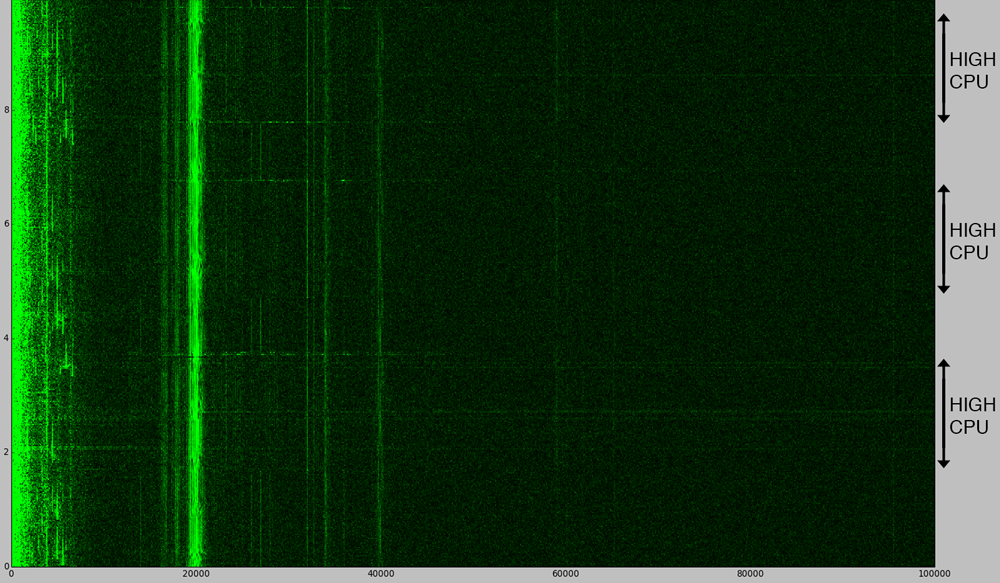
\includegraphics[width=1\linewidth]{T60p-bk-cpuload-eps-1_description.png}
	    \caption{With AC power adopter}
	    \label{fig:appendix_T60p-bk-cpuload-eps-1-1a}
    \end{subfigure}
    \begin{subfigure}{1\textwidth}
	    \centering
	    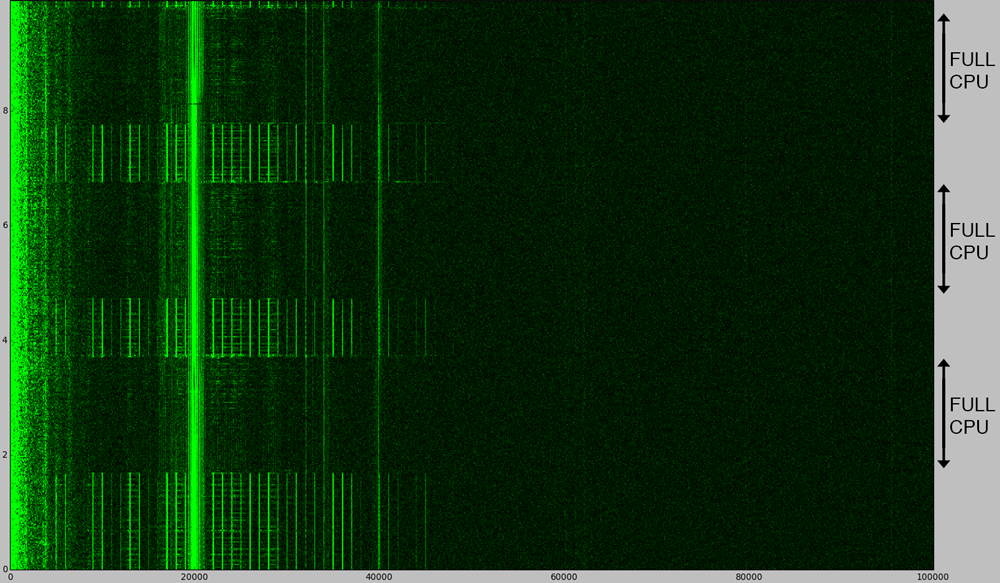
\includegraphics[width=1\linewidth]{T60p-bk-cpuload-ips-0_description.png}
	    \caption{Running on battery power}
	    \label{fig:appendix_T60p-bk-cpuload-ips-0-1b}
    \end{subfigure}
    \caption{Acoustic signature (10 sec, 0-100kHz) of the Lenovo T60p when running a high CPU load described in~\autoref{chp4:sec:cpu_load}. Recorded in an anechoic chamber using the lab-grade setup. }
	\label{fig:appendix_T60p-bk-cpuload}
\end{figure}

%=============================
% D430 Anechoic chamber  IDLE
%=============================
%The~\autoref{fig:D430-ekkofritt-bk-idle-eps-1} is the result from the running idle on the Dell 430 in the anechoic chamber. 
%\begin{figure}[ht]
%    \centering
%    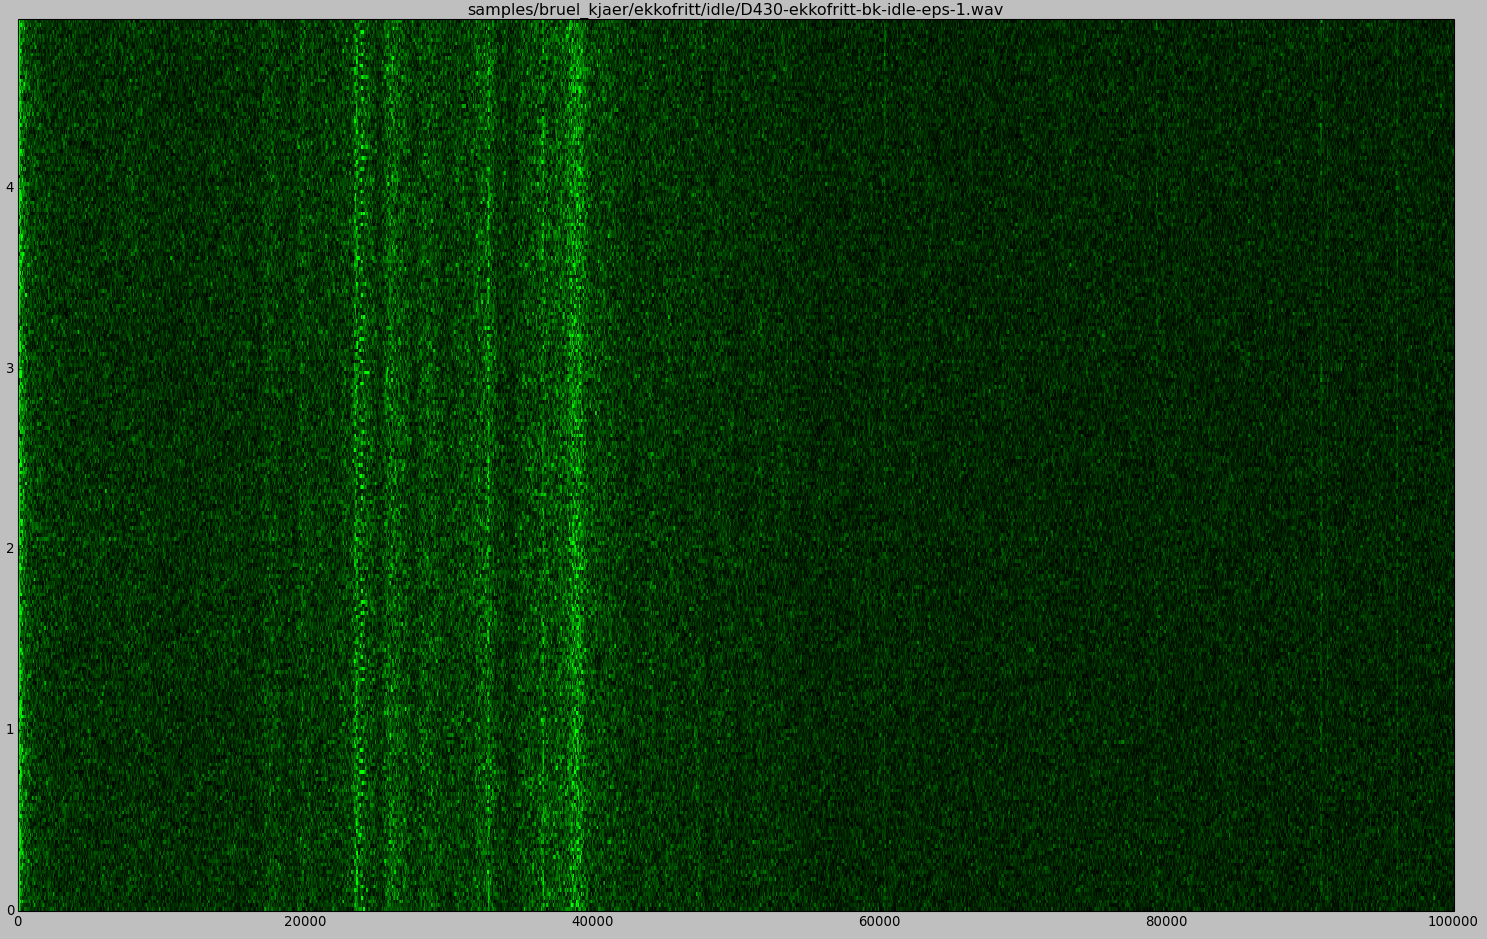
\includegraphics[width=0.7\linewidth]{D430-ekkofritt-bk-idle-eps-1.png}
%    \caption{Acoustic recording (Vertical axis: 5 sec. Horizontal axis: 0-100kHz) of the Dell D430 when idle. The recording was made in an anechoic chamber using the Brüel\&Kjær 4939 configuration specified in~\autoref{chp3:sec:bruel_kjaer_configuration}. }
%    \label{fig:D430-ekkofritt-bk-idle-eps-1}
%\end{figure}

%==============
% Raspberry PI
%==============

\section{Raspberry PI}\label{apx:sec:raspberry}
All of our recordings of the Raspberry PI is more or less equal and inconclusive, empirically speaking. 
~\autoref{fig:appendix_RB-ekkofritt-bk-micro-0} is the inconclusive result gained from running the CPU operations. 
\begin{figure}[ht]
    \centering
    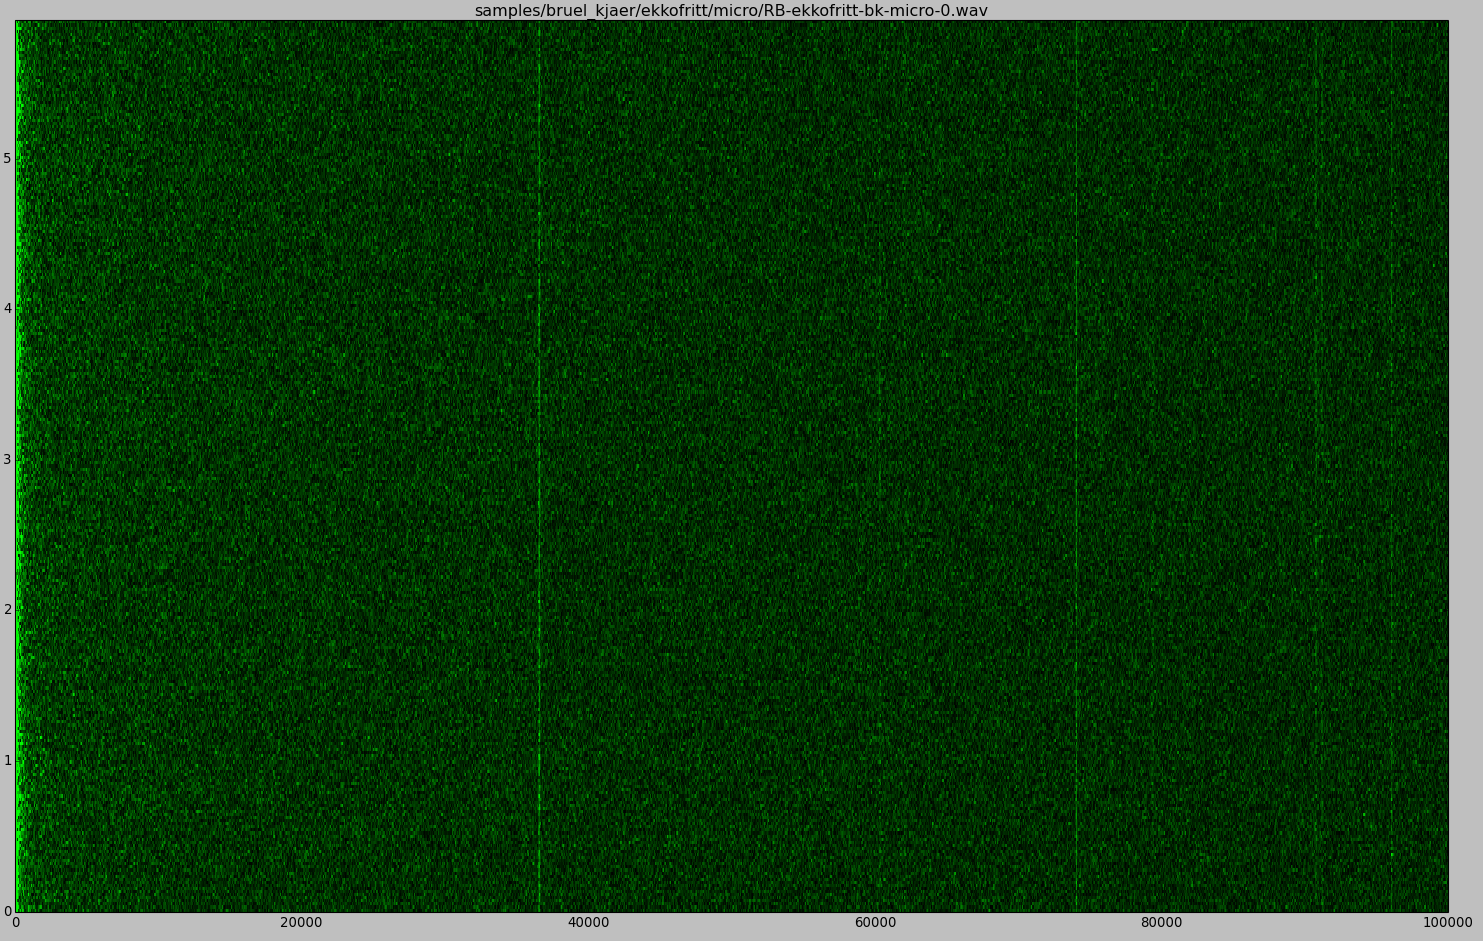
\includegraphics[width=1\linewidth]{RB-ekkofritt-bk-micro-0.png}
    \caption{Acoustic signature (6 sec, 0-100kHz) of the Raspberry PI running the CPU operations.
        Recorded in an anechoic chamber using the lab-grade setup.}
    \label{fig:appendix_RB-ekkofritt-bk-micro-0}
\end{figure}

\end{document} 
